\documentclass{ximera}

\makeatletter

\RequirePackage{sagetex}


\graphicspath{
  {./}
  {./explorePolynomials/}
  {./exploreRadicals/}
  {./graphing/}
  {./examReview}
}


%% Because log being natural log is too hard for people.
\let\logOld\log% Keep the old \log definition, just in case we need it.
\renewcommand{\log}{\ln}


\providecommand\tabitem{\makebox[1em][r]{\textbullet~}}
\providecommand{\letterPlus}{\makebox[0pt][l]{$+$}}
\providecommand{\letterMinus}{\makebox[0pt][l]{$-$}}

\renewcommand{\texttt}[1]{#1}% Renew the command to prevent it from showing up in the sage strings for some weird reason.


%%%%%%%%%%%%%%%%%%%%%%%%%%%%%%%%
%%% Randomize Locations Code %%%
%%%%%%%%%%%%%%%%%%%%%%%%%%%%%%%%

%% Required Packages
%\RequirePackage[margin=2.5cm]{geometry}% Set generic Margins to 1.5cm
\RequirePackage{fancyhdr}% Used to make header/footers
%\RequirePackage[hidelinks]{hyperref}%
%\RequirePackage{tikz, pgfplots}
\RequirePackage{forloop}
\RequirePackage{changepage}
\RequirePackage{morewrites}
\RequirePackage{calc}


%%%%%%%%%%%%%%%%%%%%%%%% End of Required Packages



%% Necessary Counters

\newcounter{choiceNum}% This will track the choice number in a given MCChoice environment.
\newcounter{choiceEnvNum}% This lets the \choice generated commands be uniquely identified to the correct MCChoice environment.
    \setcounter{choiceEnvNum}{0}% Start at 0 as we step the counter before assigning things.
\newcounter{questionNum}% Tracks what number a question is within a given MCQ environment.



% Iteration counters
\newcounter{Iteration@printChoices}
\newcounter{Iteration@questionsInBlock}
\newcounter{Iteration@printQuestions}

%% End Counters

%% New "if" commands
\newif\ifVerbose% For error Checking
\Verbosefalse

\newif\ifInner@Shuffle% If we want our vector to be shuffled
\Inner@Shufflefalse

\newif\ifInner@OrderForward% If we want non-shuffled and original order (smallest value to biggest value).
\Inner@OrderForwardfalse

\newif\ifInner@OrderReverse% If we want non-shuffled but reverse order (biggest value to smallest value).
\Inner@OrderReversefalse

\newif\ifshuffleChoices%    Toggle to shuffle choice locations.
\shuffleChoicesfalse

\newif\ifshuffleQuestions%  Toggle to shuffle Question locations.
\shuffleQuestionsfalse

\newif\ifgenAnsKey% Tracks if we want 
\genAnsKeyfalse

\newif\ifcorrectAns% This will track if a choice is correct.
\correctAnsfalse

%% End "if" commands


%%%%%%%%%%%%%%%%%%%%%%%% End of Package Options


%%% Support commands %%%
\providecommand\compareStrings[2]{% Used to compare two strings to see if they are the same - up to case sensitivity.
    \edef\tempA{\lowercase{\noexpand\ifnum0=\noexpand\pdfstrcmp
        {\noexpand\zap@space#1 \noexpand\@empty}%
        {\noexpand\zap@space#2 \noexpand\@empty}%
    }\relax}%
    \tempA
        \expandafter\@firstoftwo
    \else
        \expandafter\@secondoftwo
    \fi
}

\providecommand{\MakeCounter}[1]{%% Code located in "Utilitymacros.dtx"
  \@ifundefined{c@#1}% Check to see if counter exists
        {     % If not, create it and set it to 0.
            \newcounter{#1}
            \setcounter{#1}{0}
        }
        {%If so, reset to 0.
            \setcounter{#1}{0}
        }
    }








%%%%%%%%%%%%%%%%%%%%%%%%%%%%%%%%%%%%%%%%%%%%%%%%%%%%%%%%%%%%%%%%%%%%%
%%%%%%%%%%%%%%%%%%%		  Randomize Commands		%%%%%%%%%%%%%%%%%
%%%%%%%%%%%%%%%%%%%%%%%%%%%%%%%%%%%%%%%%%%%%%%%%%%%%%%%%%%%%%%%%%%%%%


%%%%%%%%%%%%%%%%%%%%%%%%%%%%%%%%%%%%%%%%%%%%%%%%%%%%%%%%%%%%%
%%%%%%%%%%%%  Random Permutation Command  %%%%%%%%%%%%%%%%%%%
%%%%%%%%%%%%%%%%%%%%%%%%%%%%%%%%%%%%%%%%%%%%%%%%%%%%%%%%%%%%%

\MakeCounter{RndQuant}%		        Tracks the number of desired counters
\MakeCounter{Temp@Hold}%		    Temp counter to hold the command value because tex is weird.
\MakeCounter{Temp@RandMe}%	        Temp counter like previous.

\providecommand*\ifcounter[2]{%         Function checks if a counter named #1 exists. If not it creates it. After existance is confirmed (or implemented), set the counter to #2.
  \ifcsname c@#1\endcsname
  \else
    \MakeCounter{#1}
  \fi
\setcounter{#1}{#2}
}

\providecommand{\RandMe}[3]{% #1 is the max number for range, #2 is the name of the counter to hold the list, and #3 is how many from that list to generate. Thus \RandMe{100}{TEMP}{5} will generate 5 counters, named \TEMPI, \TEMPII, \TEMPIII, \TEMPIV, \TEMPV. Each of which will have a (unique) number between 1 and 100.

    %Assign a maximum on how many numbers to pick. Set default to the max list size, and save in counter "RndQuant"
    \ifthenelse{\isempty{#3}}
        {
        \setcounter{RndQuant}{#1+1}
        }
        {
        \setcounter{RndQuant}{#3+1}
        }

    %Generate a starting list of numbers 1 to maximum number given
    \forloop{Iteration1}{1}{\arabic{Iteration1} < \arabic{RndQuant}}{
        \ifcounter{#2\Roman{Iteration1}}{\arabic{Iteration1}}
        }% End Forloop
    
    
    %Permute using Knuth method
    \forloop{Iteration1}{1}{\arabic{Iteration1} < \arabic{RndQuant}}{
        \@genrand{TempRandMe}{\arabic{Iteration1}}{#1}
    
        \ifcounter{Temp@RandMe}{\TempRandMe}
        \ifcounter{Temp@Hold}{\arabic{#2\Roman{Temp@RandMe}}}
        
        \ifcounter{#2\Roman{Temp@RandMe}}{\arabic{#2\Roman{Iteration1}}}
        \ifcounter{#2\Roman{Iteration1}}{\arabic{Temp@Hold}}
    }
}




%%%%%%%%%%%%%%%%%%%%%%%%%%%%%%%%%%%%%%%%%%%%%%%%%%%%%%%%%%%%%
%%%%%%%%%%%%  Random Permutation Command  %%%%%%%%%%%%%%%%%%%
%%%%%%%%%%%%%%%%%%%%%%%%%%%%%%%%%%%%%%%%%%%%%%%%%%%%%%%%%%%%%


\providecommand{\@genrand}[3]{%\@genrand{NAME}{MIN}{MAX} generates a random number before MIN and MAX and stores it in the command \NAME. 
    \expandafter\pgfmathrandominteger\csname #1\endcsname{#2}{#3}
    \setcounter{#1}{\csname #1\endcsname}
}




%%%%%%%%%%%%%%%%%%%%%%%%%%%%%%%%%%%%%%%%%%%%%%%%%%%%%%%%%%%%%%%%%%%%%%%%%%%%%%%
%%%%%%%%%  		Make Vector is used to generate most random lists		%%%%%%%%%
%%%%%%%%%%%%%%%%%%%%%%%%%%%%%%%%%%%%%%%%%%%%%%%%%%%%%%%%%%%%%%%%%%%%%%%%%%%%%%%

\MakeCounter{Temp@1}
\MakeCounter{Temp@2}
\MakeCounter{Temp@3}
\MakeCounter{Iteration@1}
\MakeCounter{Iteration@2}
\MakeCounter{Iteration@3}
\MakeCounter{Iteration@4}
\MakeCounter{Placement@1}
\setcounter{Placement@1}{1}



%%%%%%%% Internal Keys
%% These are to use for internal flags only.
\providecommand{\inner@SetKeys}[1]{
\setkeys{key@Inner}{InnerShuffle={}, Order@Direction={},#1}
}


\define@key{key@Inner}{InnerShuffle}{% This flag is for shuffling questions.
\ifthenelse{\equal{#1}{true}}
	{
	\Inner@Shuffletrue
	}
	{
	\Inner@Shufflefalse
	}
}

\define@key{key@Inner}{Order@Direction}{% This flag gives the order in which vectors are saved.
\ifthenelse{\equal{#1}{forward}}
	{
	\Inner@OrderForwardtrue
	}
	{
	\Inner@OrderForwardfalse
	}
\ifthenelse{\equal{#1}{reverse}}
	{
	\Inner@OrderReversetrue
	}
	{
	\Inner@OrderReversefalse
	}
}



\providecommand{\make@Vector}[5][InnerShuffle=false, Order@Direction=forward]{% This is to make either an ordered or a shuffled list of values
	% #1 is optional and is for internal flags. 
	% #2 is the name of the output counters
	% #3 is the minimum counter value
	% #4 is the maximum counter value
	% #5 is the number of desired counters.
	% Counters will be saved as #2\Roman{#}
	
	\inner@SetKeys{#1}% Set any given keys
	% Possible flags:
		% InnerShuffle flag "true" will shuffle, "false" won't
		% Order@Direction; "forward" will list questions in increasing order. "reverse" will list the questions in 					decreasing order
		% 
	
%%%%%%%%%%%%%%%%%%%%%%%%%%%%%%%%%%%%%%%%%%%%%%%%%%%%%%%%%%%%%%%%%%%%%%%%%%%%%%%
%%%%%%%%%  		First we will choose and order the initial values		%%%%%%%%%
%%%%%%%%%%%%%%%%%%%%%%%%%%%%%%%%%%%%%%%%%%%%%%%%%%%%%%%%%%%%%%%%%%%%%%%%%%%%%%%
	\setcounter{Temp@1}{#4}
	\addtocounter{Temp@1}{-#3}
	\ifnum #5 = \value{Temp@1}% The special case where we want all the values. Randomizing into a full list just to order it is silly so we deal with this case separately.
		\forloop{Iteration@1}{1}{\arabic{Iteration@1} < \arabic{Temp@1}}
			{% Start of forloop
			\MakeCounter{Ordered@\Roman{Iteration@1}}	% Check to see if counter exists
			\MakeCounter{C@Shuffle\Roman{Iteration@1}}
			\setcounter{Ordered@\Roman{Iteration@1}}{\arabic{Iteration@1}}
			\setcounter{C@Shuffle\Roman{Iteration@1}}{\arabic{Iteration@1}}
			}
	\else% If we don't want a full list, then we need to choose some.
		\setcounter{Temp@1}{#5}% Track how many numbers we want.
		\stepcounter{Temp@1}% Step for the < sign
		\forloop{Iteration@1}{1}{\arabic{Iteration@1} < \arabic{Temp@1}}
			{% Start of forloop
	
			\MakeCounter{Ordered@\Roman{Iteration@1}}	% Check to see if counter exists
			\MakeCounter{CTemp\Roman{Iteration@1}}	% Check to see if counter exists
			\MakeCounter{C@Shuffle\Roman{Iteration@1}}
		
			\@genrand{Temp@2}{#3}{#4}
			\ifVerbose{Your first choice for the question number is \arabic{Temp@2}}\\ \fi
			\forloop{Iteration@2}{1}{\arabic{Iteration@2} < \arabic{Iteration@1}}
				{% Start of inner forloop. This loop checks for uniqueness of counter value.
				\ifnum\value{Temp@2}=\value{CTemp\Roman{Iteration@2}}% Check to see if the counter matches any previous counter
				\@genrand{Temp@2}{#3}{#4}% If so, fix it.
				\setcounter{Iteration@2}{0}% Reset the check counter so we can check if the new number is used.
				\ifVerbose Your revised choice for the number is \arabic{Temp@2} \\ \fi
				\fi
	%			\arabic{Iteration@2}, \arabic{CTemp\Roman{Iteration@2}}\\
				}% 
			
			\setcounter{CTemp\Roman{Iteration@1}}{\arabic{Temp@2}}% Save (unsorted) unique value in a temp list of variables.
			\setcounter{C@Shuffle\Roman{Iteration@1}}{\arabic{Temp@2}}% Save (unsorted) unique value in a temp list of variables. This one is to be used in the case we want shuffled values at the end.
		
			\ifVerbose (Unordered) We want questions number \arabic{Temp@2} \fi
		
			}
		% Now we want to sort the list	
	
		\forloop{Iteration@3}{1}{\arabic{Iteration@3}<\arabic{Temp@1}}
			{% For each variable
				\setcounter{Placement@1}{1}% Default the placeholder counter to some gigantic number so I can proceed to find the smallest possible number.
			
				\forloop{Iteration@4}{1}{\arabic{Iteration@4}<\arabic{Temp@1}}
					{
					\ifnum\value{CTemp\Roman{Iteration@4}}<\value{CTemp\Roman{Placement@1}}
						\setcounter{Placement@1}{\arabic{Iteration@4}}% Keep track of which counter was the largest so far
					\fi
					}
	
				\setcounter{Ordered@\Roman{Iteration@3}}{\arabic{CTemp\Roman{Placement@1}}}% Set the final counter.
				\setcounter{CTemp\Roman{Placement@1}}{999999}% Now remove that place as a viable option for next run.
				\ifVerbose (Ordered) We want question number \arabic{Ordered@\Roman{Iteration@3}} \fi
			}
	\fi	
%%%%%%%%%%%%%%%%%%%%%%%%%%%%%%%%%%%%%%%%%%%%%%%%%%%%%%%%%%%%%%%%%%%%%%%%%%%%%%%	
%%%%%%%%%%%		Finished Choosing and ordering initial values		%%%%%%%%%%%
%%%%%%%%%%%%%%%%%%%%%%%%%%%%%%%%%%%%%%%%%%%%%%%%%%%%%%%%%%%%%%%%%%%%%%%%%%%%%%%
%%%%%%%%%%%   		Now reorder and assign final names				%%%%%%%%%%%
%%%%%%%%%%%%%%%%%%%%%%%%%%%%%%%%%%%%%%%%%%%%%%%%%%%%%%%%%%%%%%%%%%%%%%%%%%%%%%%
	
	
	\ifInner@OrderReverse
		\setcounter{Temp@3}{#5}
		\forloop{Iteration@1}{1}{\arabic{Iteration@1} < \arabic{Temp@1}}
			{
			\MakeCounter{#2\Roman{Iteration@1}}% Make the counter if it doesn't exist.
			\setcounter{#2\Roman{Iteration@1}}{\arabic{Ordered@\Roman{Temp@3}}}% Set the final counter version to the current "last" unused value.
			\addtocounter{Temp@3}{-1}% Decrement the counter for next assignment
			}
	\else% If we aren't doing it in reverse, assume we want forward order. This is default.
		\forloop{Iteration@1}{1}{\arabic{Iteration@1} < \arabic{Temp@1}}
			{
			\MakeCounter{#2\Roman{Iteration@1}}% Make the counter if it doesn't exist.
			\setcounter{#2\Roman{Iteration@1}}{\arabic{Ordered@\Roman{Iteration@1}}}% Set the final counter version to the next value.
			}
	
	\fi% End of forward/reverse order version

	\ifInner@Shuffle
		\forloop{Iteration@1}{1}{\arabic{Iteration@1} < \arabic{Temp@1}}
			{
			\MakeCounter{#2\Roman{Iteration@1}}% Make the counter if it doesn't exist.
			\setcounter{#2\Roman{Iteration@1}}{\arabic{C@Shuffle\Roman{Iteration@1}}}% Set the counter to the next value.
			}

	\fi% End of Shuffle order version
	
}


%%%%%%%%%%%%%%%%%%%%%%%%%%%%%%%%%%%%%%%%%%%%%%%%%%%%%%%%%%%%%%%%%%%%%%%%%%%%%%%%%%%%%%%%%%%%%%%%%%%%
%%%%%%%%%%%%%%%%%%%%%%%%%               Shuffle Structure               %%%%%%%%%%%%%%%%%%%%%%%%%%%%
%%%%%%%%%%%%%%%%%%%%%%%%%%%%%%%%%%%%%%%%%%%%%%%%%%%%%%%%%%%%%%%%%%%%%%%%%%%%%%%%%%%%%%%%%%%%%%%%%%%%
%%%%% Structure of randomizing/printing problems and choices:
%    All the MC questions are wrapped in an environment, eg MCQuestions. 
%        At the termination of the block, the questions are printed. This will determine shuffling.
%    We use a \questionblock type command to save questions together that need to be put together. 
%        eg questions that have a ``use the following information for the next 3 problems.''
%        \shuffleblock takes an argument that denotes how many sub-questions are contained in a block.
%    We use a \question command to save the content of a question into a macro.
%    Each individual MC question uses a choices environment and choices command as the \item equivalent.
%        The termination of the choices environment will shuffle (or not) the choices.
%
%    When we print the problems, we will iterate through the question content and/or the shuffleblocks
%        If a shuffle block has too many questions in it for how many ``more'' questions we want, we skip it.
%        Print things in order (or random order) until we have however many questions we want.
%            BADBAD:: If you randomize the questions just right with larger shuffle blocks at the end;
%                it's possible that the number of problems printed won't be the desired amount, even if there
%                are enough problems in the bank. We can get around this by changing the seed in the short term.
    


%%%%%%%%%%%%%%%%%%%%%%%%%%%%%%%%%%%%%%%%%%%%%%%%%%%%%%%%%%%%%%%%%%%%%%%%%%%%%%%%%%%%%%%%%%%%%%%%%%%%
%%%%%%%%%%%%%%%%%%%%%%%%%       Question Environments and Commands      %%%%%%%%%%%%%%%%%%%%%%%%%%%%
%%%%%%%%%%%%%%%%%%%%%%%%%%%%%%%%%%%%%%%%%%%%%%%%%%%%%%%%%%%%%%%%%%%%%%%%%%%%%%%%%%%%%%%%%%%%%%%%%%%%

%% MCQuestions Environment
\newcounter{MCquestionPrint}% Counter to save how many questions we want to print from the MCQ environment.

\newenvironment{MCQuestions}[1][1000]% Use massive default number to print all problems if none is given.
    {% Start environment code
        \setcounter{MCquestionPrint}{#1}%   Save how many questions we want from this environment to a counter.
    }% End start environment code
    {% End environment code
        {\expandafter\printQuestions{\arabic{MCquestionPrint}}}%
    }% End of end environment code.





%%% Defining the questionblock command.
\newif\ifquestionBlock%     We define a flag so we know if we are in a question block.
\questionBlockfalse%        We will assume that, by default, we are not in a question block.
\newcounter{shuffleNum}%    This will track how many blocks are present to shuffle.
\setcounter{shuffleNum}{0}%    Start at zero.
%\newcounter{blockNum}%      A counter to track which block number we are on.
%\setcounter{blockNum}{0}%   By default we haven't iterated a block yet.

\providecommand{\questionBlock}[2]{%    This is a command that should allow one to group together a block of questions, 
%                                            in order, to be considered one ``big question'' for the purposes of shuffle.
%                                        Syntax: #1 is the number of questions in the block
%                                                #2 is the actual content of the block, eg the questions.
    \stepcounter{shuffleNum}%                                   We have started a question block, so we iterate the shuffleNum to know we aim to shuffle this as one block. 
    \expandafter\MakeCounter{Block\roman{shuffleNum}Size}%      Create a counter to hold how many questions are in this block.
    \expandafter\setcounter{Block\roman{shuffleNum}Size}{#1}%   And record how many questions are in this block.
    \ifpoolProblem
        \stepcounter{poolPlacement}% Step this counter once to say we're adding one placement into the pool.
    \fi
    
    \expandafter\gdef\csname blockPosition\roman{shuffleNum}\endcsname{
        \questionBlocktrue% We are now in a question block, so we set the flag to true. 
    %                           This should change the ``\question" behavior to just display the questions.
        #2
        \questionBlockfalse% Toggle off the shuffle block once we have spit out the problems.
        }

}% End questionBlock definition

\DeclareRobustCommand{\question}[1]{ \begin{problem} #1 \end{problem}}


%% Defining the \question command.
\DeclareRobustCommand{\question}[1]{% Question command should contain a question to be formatted.
        \ifquestionBlock
        % If it's just a block on its own, then we just group them together as one large question and call it a day.
            \begin{problem} #1\end{problem}
        \else
            \stepcounter{shuffleNum}% A new question means we need to step current shuffle number count (before definition since counter starts at 0)
            \expandafter\gdef\csname blockPosition\roman{shuffleNum}\endcsname{\begin{problem} #1 \end{problem}}
        \fi
    
    }% End \question code


%% Define the print questions command.
\newcounter{questionsPrintNum}
\setcounter{questionsPrintNum}{0}
\providecommand{\printQuestions}[1]{% This is a command that will print questions that were defined in the current question environment.
    %First, we make the call the shuffle vector based on if we are shuffling these or not.
        \ifshuffleQuestions%                    If we are shuffling, then shuffle up the call
            \make@Vector[InnerShuffle=true]{questionLoc}{1}{\arabic{shuffleNum}}{\arabic{shuffleNum}}
        \else%                                  Otherwise, display them in original first to last order.
            \make@Vector[InnerShuffle=false,Order@Direction=forward]{questionLoc}{1}{\arabic{shuffleNum}}{\arabic{shuffleNum}}
        \fi	


    	\setcounter{questionsPrintNum}{#1}%     Record how many problems we need to print.
        \stepcounter{questionsPrintNum}%        The ifthenelse doesn't like <=, so we step the counter to avoid this problem.
        \stepcounter{shuffleNum}%               The forloop doesn't like <=, so we step the counter to avoid this problem.
    	% Now print the results:
        
        \forloop{Iteration@printQuestions}{1}{\arabic{Iteration@printQuestions}<\arabic{shuffleNum}}{% Begin forloop
            % Now we need to see if we need to print the next shuffle problem.
            %% First check to see if the next shuffle item is a question block by seeing if the block num counter is defined.
            \ifcsname c@Block\roman{questionLoc\Roman{Iteration@printQuestions}}Size\endcsname
                % If the counter is defined, then the next item is a question block and the counter is the number of questions.
                \ifthenelse{ \arabic{Block\roman{questionLoc\Roman{Iteration@printQuestions}}Size} < \arabic{questionsPrintNum}}
                    {% If the block is small enough, then go ahead and print them.
                        \ifVerbose Printing question block labeled: blockPosition\roman{questionLoc\Roman{Iteration@printQuestions}}...\fi
                        
                        \csname blockPosition\roman{questionLoc\Roman{Iteration@printQuestions}}\endcsname%
                        %   And, since we printed them, we need fewer problems to print!
                        \addtocounter{questionsPrintNum}{-\arabic{Block\roman{questionLoc\Roman{Iteration@printQuestions}}Size}}
                        
                        \ifVerbose Now we have \thequestionsPrintNum more questions to go...\fi
                    }
                    {% Otherwise, do nothing.
                        Tried to print a question block but it didn't fit...
                    }
            \else% Otherwise the next item is just a singleton question.
                %Printing question labeled: blockPosition\roman{questionLoc\Roman{Iteration@printQuestions}}
                
                \csname blockPosition\roman{questionLoc\Roman{Iteration@printQuestions}}\endcsname%
                \addtocounter{questionsPrintNum}{-1}% We printed a question, so there's one fewer needed to print.
                
                %Now we have \thequestionsPrintNum more questions to go...
            \fi
            %% Finally, we will check if we still need to use this for loop.
            \ifthenelse{\arabic{questionsPrintNum} < 2}{% If the questionsPrint is less than 2 (since we stepped the counter), then we are done.
            \setcounter{Iteration@printQuestions}{\arabic{shuffleNum}}% Breakout of the forloop.
            \ifVerbose And we're done.\fi
            }
            {% If we aren't done, then do nothing with this check.
            \ifVerbose Keep going, we haven't stopped yet...\fi
            }
        }% End forloop
        %\addtocounter{shuffleNum}{-1}% Undo the stepcounter to be safe.
    }% End \printQuestions code.


%%%%%%% Choices Code

%\let\choiceOnline\choice% Define the old online choice command as the generic ``choice'' command; we'll see what happens.
\providecommand{\choiceShuffle}[2][]{% Choice command holds a multiple choice option by generating a new command with unique name that will be used to write the outputs at the end of the MCChoices environment.
            \refstepcounter{choiceNum}% A new choice means we need to step current choice (before definition since counters starts at 0)
            \expandafter\gdef\csname \Roman{choiceEnvNum}choice\roman{choiceNum}\endcsname{\choice[#1]{#2}}
        }% End of \choice code.
        
%%% Choice environment just collects and prints choices for each one locally.
\newenvironment{choices}{% Start environment code for multiple choice Choices environment
        \setcounter{choiceNum}{0}% New MCChoices environment means a new set of choices, so reset current choice to 0.
        \refstepcounter{choiceEnvNum}
    }% End of end-environment code.
    {
    \printChoices
    }



\renewcommand{\thechoiceEnvNum}{\Roman{choiceEnvNum}}
\renewcommand{\thechoiceNum}{\Alph{choiceNum}}
\renewcommand{\theIteration@printChoices}{\Alph{Iteration@printChoices}}

\providecommand{\printChoices}{% \printChoices is an internal macro to print the choices at the end of a MCChoice environment, depending on if we want them shuffled or not.

    %First, we make the call vector based on if we are shuffling these or not.
    \ifshuffleChoices% If we are shuffling, then shuffle up the call
        \make@Vector[InnerShuffle=true]{choiceLoc}{1}{\arabic{choiceNum}}{\arabic{choiceNum}}
    \else% Otherwise, display them in original first to last order.
        \make@Vector[InnerShuffle=false, Order@Direction=forward]{choiceLoc}{1}{\arabic{choiceNum}}{\arabic{choiceNum}}
    \fi	
    
	% Now print the results:
	
    \stepcounter{choiceNum}% Step counter for the < symbol in foreloop.
    
    \ifVerbose I think my choice number is \thechoiceNum{} and my choice env is \thechoiceEnvNum{}\fi
    \begin{multipleChoice}
        \forloop{Iteration@printChoices}{1}{\arabic{Iteration@printChoices}<\arabic{choiceNum}}{% Begin forloop
                \csname \thechoiceEnvNum choice\expandafter\roman{choiceLoc\Roman{Iteration@printChoices}}\endcsname
            }% End For Loop
    \end{multipleChoice}
    }% End of \printChoices code.











\title{Exam One Review}


\begin{document}
\begin{abstract}
This is a (lengthy) practice exam for Exam 1.
\end{abstract}
\maketitle

\shuffleChoicestrue
\shuffleQuestionstrue
\pgfmathsetseed{581}

\textbf{NOTE:} There may be random lines that look like \verb|\texttt{(SOME TEXT)}| and maybe even some \verb|{ }| within that text. You can ignore everything that isn't the text itself; ie the texttt bit and the braces, they are an artifact of how some randomization is being done that I haven't had time to fix yet. If you literally delete the \verb|\texttt| and the braces from what you see, and just keep the text itself, it will read exactly as intended. So just ignore all those texttt and braces whenever you see them.

Also note: Some of the below has randomized elements, some do not. Currently Xronos does not support randomized graphing (although we're working on it!) so a lot of the graphing problems won't randomize, but a surprising amount of the other problems will change values or text if you hit the green ``another'' button in the top right corner to get another version of this practice exam. This also means it may take some time for the entire test to render because we have to rely on public servers to do the randomization for us currently, so please be patient. If it takes more than 3-5 minutes to fill out the random values (meaning: if there are still spinning wheels of death going after 3-5 minutes) there is a problem. Try hitting the ``another'' button to see if it resolves itself. If it keeps doing this, please contact your instructor and let him know!

\begin{sagesilent}
def RandInt(a,b):
    """ Returns a random integer in [`a`,`b`]. Note that `a` and `b` should be integers themselves to avoid unexpected behavior.
    """
    return QQ(randint(int(a),int(b)))
    # return choice(range(a,b+1))

def NonZeroInt(b,c, avoid = [0]):
    """ Returns a random integer in [`b`,`c`] which is not in `av`. 
        If `av` is not specified, defaults to a non-zero integer.
    """
    while True:
        a = RandInt(b,c)
        if a not in avoid:
            return a

algHans1 = 0
algHans2 = 0
algHans3 = 0
algHans4 = 0
algHans5 = 0

while algHans1 == algHans2 or algHans1 == algHans3 or algHans1 == algHans4 or algHans1 == algHans5 or algHans2 == algHans3 or algHans2 == algHans4 or algHans2 == algHans5 or algHans3 == algHans4 or algHans3 == algHans5 or algHans4 == algHans5:
    algHc1 = RandInt(-5,5)
    algHc2 = RandInt(-5,5)
    algHc3 = RandInt(-5,5)
    algHc4 = NonZeroInt(-5,5)
    algHfuncvec = [x, x^2, x^3]
    algHpick1 = RandInt(0,2)
    algHpick2 = RandInt(0,2)
    algHpick3 = RandInt(0,2)
    
    algHfunc1 = algHfuncvec[algHpick1] + algHc2
    algHfunc2 = algHfuncvec[algHpick2] + algHc3
    algHfunc3 = algHfuncvec[algHpick3] + algHc4
    
    algHans1 = algHfunc1(algHc1)*(algHfunc2(algHc1)-algHfunc3(algHc1))
    algHans2 = algHfunc1(algHc1)*(algHfunc2(algHc1)-algHfunc3(algHc1) + 2*algHc4)
    algHans3 = algHfunc1(algHc1)*algHfunc2(algHc1)-algHfunc3(algHc1)
    algHans4 = algHfunc1(algHc1)*algHfunc2(algHc1)-algHfunc3(algHc1) + 2*algHc4
    algHans5 = algHfunc1(algHc1)*(algHfunc2(algHc1)+algHfunc3(algHc1))

\end{sagesilent}


\begin{MCQuestions}
\question{
    Suppose $f(x) = \sage{algHfunc1}$, $g(x) = \sage{algHfunc2}$, and $h(x) = \sage{algHfunc3}$; compute $(f\cdot(g-h))(\sage{algHc1})$.

    \begin{choices}
        \choiceShuffle[correct]{$\sage{algHans1}$}
        \choiceShuffle{$\sage{algHans2}$}
        \choiceShuffle{$\sage{algHans3}$}
        \choiceShuffle{$\sage{algHans4}$}
        \choiceShuffle{$\sage{algHans5}$}
    \end{choices}
}



\begin{sagesilent}
#### Problem p1
compEans1 = 0
compEans2 = 0
compEans3 = 0
compEans4 = 0
compEans5 = 0

while compEans1 == compEans2 or compEans1 == compEans3 or compEans1 == compEans4 or compEans1 == compEans5 or compEans2 == compEans3 or compEans2 == compEans4 or compEans2 == compEans5 or compEans3 == compEans4 or compEans3 == compEans5 or compEans4 == compEans5:
    compEc1 = RandInt(-5,5)
    compEfuncvec = [x, x^2, x^3]
    compEpick1 = RandInt(0,2)
    compEpick2 = RandInt(0,2)
    
    compEfunc1 = compEfuncvec[compEpick1] + RandInt(-5,5)
    compEfunc2 = compEfuncvec[compEpick2] + RandInt(-5,5)
    
    compEans1 = compEfunc1(compEfunc2(compEc1))
    compEans2 = compEfunc2(compEfunc1(compEc1))
    compEans3 = -compEfunc1(compEfunc2(compEc1))
    compEans4 = compEfunc1(compEc1) * compEfunc2(compEc1)
    compEans5 = compEfunc1(compEc1) + compEfunc2(compEc1)

\end{sagesilent}



\question{
    Suppose $f(x) = \sage{compEfunc1}$ and $g(x) = \sage{compEfunc2}$; compute $(f \circ g)(\sage{compEc1})$.

    \begin{choices}
        \choiceShuffle[correct]{$\sage{compEans1}$}
        \choiceShuffle{$\sage{compEans2}$}
        \choiceShuffle{$\sage{compEans3}$}
        \choiceShuffle{$\sage{compEans4}$}
        \choiceShuffle{$\sage{compEans5}$}
    \end{choices}
}





\begin{sagesilent}
#### Problem p1algE
p1algEans1 = 0
p1algEans2 = 0
p1algEans3 = 0
p1algEans4 = 0
p1algEans5 = 0

while p1algEans1 == p1algEans2 or p1algEans1 == p1algEans3 or p1algEans1 == p1algEans4 or p1algEans1 == p1algEans5 or p1algEans2 == p1algEans3 or p1algEans2 == p1algEans4 or p1algEans2 == p1algEans5 or p1algEans3 == p1algEans4 or p1algEans3 == p1algEans5 or p1algEans4 == p1algEans5:
    p1algEc1 = RandInt(-5,5)
    p1algEc2 = RandInt(-5,5)
    p1algEc3 = RandInt(-5,5)
    p1algEfuncvec = [x, x^2, x^3]
    p1algEpick1 = RandInt(0,2)
    p1algEpick2 = RandInt(0,2)
    
    p1algEfunc1 = p1algEfuncvec[p1algEpick1] + p1algEc2
    p1algEfunc2 = p1algEfuncvec[p1algEpick2] + p1algEc3
    
    p1algEans1 = p1algEfunc1(p1algEc1) - p1algEfunc2(p1algEc1)
    p1algEans2 = p1algEfunc1(p1algEc1) + p1algEfunc2(p1algEc1)
    p1algEans3 = p1algEfunc1(p1algEc1) - p1algEfunc2(p1algEc1) + 2*p1algEc3
    p1algEans4 = p1algEfunc1(p1algEc1)*p1algEfunc2(p1algEc1)
    p1algEans5 = p1algEfunc1(p1algEfunc2(p1algEc1))




#### Problem p2algE
p2algEans1 = 0
p2algEans2 = 0
p2algEans3 = 0
p2algEans4 = 0
p2algEans5 = 0

while p2algEans1 == p2algEans2 or p2algEans1 == p2algEans3 or p2algEans1 == p2algEans4 or p2algEans1 == p2algEans5 or p2algEans2 == p2algEans3 or p2algEans2 == p2algEans4 or p2algEans2 == p2algEans5 or p2algEans3 == p2algEans4 or p2algEans3 == p2algEans5 or p2algEans4 == p2algEans5:
    p2algEc1 = x
    p2algEc2 = RandInt(-5,5)
    p2algEc3 = RandInt(-5,5)
    p2algEfuncvec = [x, x^2, x^3]
    p2algEpick1 = RandInt(0,2)
    p2algEpick2 = RandInt(0,2)
    
    p2algEfunc1 = p2algEfuncvec[p2algEpick1] + p2algEc2
    p2algEfunc2 = p2algEfuncvec[p2algEpick2] + p2algEc3
    
    p2algEans1 = p2algEfunc1(p2algEc1) - p2algEfunc2(p2algEc1)
    p2algEans2 = p2algEfunc1(p2algEc1) + p2algEfunc2(p2algEc1)
    p2algEans3 = p2algEfunc1(p2algEc1) - p2algEfunc2(p2algEc1) + 2*p2algEc3
    p2algEans4 = expand(p2algEfunc1(p2algEc1)*p2algEfunc2(p2algEc1))
    p2algEans5 = p2algEfunc1(p2algEfunc2(p2algEc1))





\end{sagesilent}



\question{ 
    Suppose $f(x) = \sage{p1algEfunc1}$, $g(x) = \sage{p1algEfunc2}$; compute $(f - g)(\sage{p1algEc1})$.

    \begin{choices}
        \choiceShuffle[correct]{$\sage{p1algEans1}$}
        \choiceShuffle{$\sage{p1algEans2}$}
        \choiceShuffle{$\sage{p1algEans3}$}
        \choiceShuffle{$\sage{p1algEans4}$}
        \choiceShuffle{$\sage{p1algEans5}$}
    \end{choices}
}


\question{ 
     Suppose $f(x) = \sage{p2algEfunc1}$, $g(x) = \sage{p2algEfunc2}$; compute $(f - g)(\sage{p2algEc1})$.

    \begin{choices}
        \choiceShuffle[correct]{$\sage{p2algEans1}$}
        \choiceShuffle{$\sage{p2algEans2}$}
        \choiceShuffle{$\sage{p2algEans3}$}
        \choiceShuffle{$\sage{p2algEans4}$}
        \choiceShuffle{$\sage{p2algEans5}$}
    \end{choices}
}



    



\begin{sagesilent}

##### Problem p1algM
p1algMans1 = 0
p1algMans2 = 0
p1algMans3 = 0
p1algMans4 = 0
while p1algMans1 == p1algMans2 or p1algMans1 == p1algMans3 or p1algMans1 == p1algMans4 or p1algMans2 == p1algMans3 or p1algMans2 == p1algMans4 or p1algMans3 == p1algMans4:
    p1algMx1 = RandInt(-5,5)
    p1algMx2 = NonZeroInt(-5,5,[p1algMx1])
    p1algMx3 = NonZeroInt(-5,5,[p1algMx1,p1algMx2])
    
    p1algMy1 = RandInt(-10,10)
    p1algMy2 = RandInt(-10,10)
    p1algMy3 = NonZeroInt(-10,10)
    
    p1algMans1 = p1algMy2*p1algMy3
    p1algMans2 = p1algMy1
    p1algMans3 = p1algMy2-p1algMy3
    p1algMans4 = p1algMy2 + p1algMy3



##### Problem p2algM
p2algMc1 = NonZeroInt(-5,5)
p2algMc2 = NonZeroInt(-5,5, [0,p2algMc1])
p2algMfuncvec = [x, x^2, x^3]
p2algMpick1 = RandInt(0,2)
p2algMf1 = p2algMfuncvec[p2algMpick1]

p2algMans1 = p2algMf1(x-p2algMc1) + p2algMc2
p2algMansfalse1 = p2algMf1(x) + p2algMc2 - p2algMc1
p2algMansfalse2 = p2algMf1(x) + p2algMc2
p2algMansfalse3 = p2algMf1(x) - p2algMc1
p2algMansfalse4 = p2algMf1(x + p2algMc1) + p2algMc2




##### Problem p3algM





\end{sagesilent}



\question{
    Given: $f(\sage{p1algMx1})=\sage{p1algMy1}$, \hfill $f(\sage{p1algMx2})=\sage{p1algMy2}$, \hfill $g(\sage{p1algMx2})=\sage{p1algMy3}$, \hfill $g(\sage{p1algMx3})=\sage{p1algMx1}$ \hfill Compute: \hspace*{2cm}
    \begin{enumerate}
    \item[a.] $(fg)(\sage{p1algMx2})$
    \item[b.] $(f\circ g)(\sage{p1algMx3})$
    \item[c.] $(f-g)(\sage{p1algMx2})$
    \end{enumerate}
    \begin{choices}
        \choiceShuffle[correct]{$(fg)(\sage{p1algMx2}) = \sage{p1algMans1}$, $(f \circ g)(\sage{p1algMx3}) = \sage{p1algMans2}$, $(f-g)(\sage{p1algMx2}) = \sage{p1algMans3}$ }
        \choiceShuffle{$(fg)(\sage{p1algMx2}) = \sage{p1algMans2}$, $(f \circ g)(\sage{p1algMx3}) = \sage{p1algMans3}$, $(f-g)(\sage{p1algMx2}) = \sage{p1algMans3}$ }
        \choiceShuffle{$(fg)(\sage{p1algMx2}) = \sage{p1algMans1}$, $(f \circ g)(\sage{p1algMx3}) = \sage{p1algMans2}$, $(f-g)(\sage{p1algMx2}) = \sage{p1algMans4}$ }
        \choiceShuffle{$(fg)(\sage{p1algMx2}) = \sage{p1algMans2}$, $(f \circ g)(\sage{p1algMx3}) = \sage{p1algMans2}$, $(f-g)(\sage{p1algMx2}) = \sage{p1algMans4}$ }
        \choiceShuffle{$(fg)(\sage{p1algMx2}) = \sage{p1algMans2}$, $(f \circ g)(\sage{p1algMx3}) = \sage{p1algMans2}$, $(f-g)(\sage{p1algMx2}) = \sage{p1algMans3}$ }
    \end{choices}
    }

\question{
    Given: $f(x) = \sage{p2algMf1}$ and $g(x) = \sage{x +p2algMc2}$. Which of the following is equivalent to $(g\circ f)(\sage{x-p2algMc1})$
    \begin{choices}
        \choiceShuffle[correct]{$\sage{p2algMans1}$}
        \choiceShuffle{$\sage{p2algMansfalse1}$}
        \choiceShuffle{$\sage{p2algMansfalse2}$}
        \choiceShuffle{$\sage{p2algMansfalse3}$}
        \choiceShuffle{$\sage{p2algMansfalse4}$}
    \end{choices}
    }

\question{
    If a function is invertible, then $f$ and $f^{-1}$ \textit{must} have the same parent function.
    \begin{choices}
        \choiceShuffle[correct]{False, it is possible for a function and its inverse to have different parent functions.}
        \choiceShuffle{True, but only if $f^{-1}$ is actually a true inverse.}
        \choiceShuffle{This is true even for partial inverses.}
        \choiceShuffle{This is false, but only because $f^{-1}$ is invertible.}
        \choiceShuffle{This would be true, but only for (all) \textit{partial} inverse functions.}
    \end{choices}
    }


\begin{sagesilent}

###### p1inverseH
p1inverseHx = 0
p1inverseHy = 0
p1inverseHxfalse = 0
p1inverseHyfalse = 0

while p1inverseHyfalse == p1inverseHxfalse or p1inverseHyfalse == p1inverseHy or p1inverseHyfalse == p1inverseHx or p1inverseHxfalse == p1inverseHx or p1inverseHxfalse == p1inverseHy or p1inverseHy == p1inverseHx:
    p1inverseHc1 = RandInt(-5,5)
    p1inverseHc2 = NonZeroInt(-5,5,[p1inverseHc1])
    p1inverseHc3 = NonZeroInt(-5,5)
    p1inverseHc4 = NonZeroInt(-5,5)
    p1inverseHc5 = NonZeroInt(-5,5)
    p1inverseHc6 = NonZeroInt(-5,5)
    
    p1inverseHf1 = p1inverseHc3*x-p1inverseHc4
    
    p1inverseHx = p1inverseHc2*p1inverseHc5 + p1inverseHc6
    p1inverseHy = (p1inverseHc1+p1inverseHc4)/p1inverseHc3
    
    p1inverseHxfalse = p1inverseHc2/p1inverseHc5 + p1inverseHc6
    p1inverseHyfalse = p1inverseHc1*p1inverseHc3 - p1inverseHc3



\end{sagesilent}



\question{
    If the point $(\sage{p1inverseHc1},\sage{p1inverseHc2})$ is on the graph of $f(x)$, then which point is on the graph of $g^{-1}(x)$ (the graph of $g$ inverse) where $g(x) = \sage{p1inverseHc5}f(\sage{p1inverseHf1}) + (\sage{p1inverseHc6})$?
    \begin{choices}
        \choiceShuffle[correct]{$(\sage{p1inverseHx},\sage{p1inverseHy})$}
        \choiceShuffle{$(\sage{p1inverseHy},\sage{p1inverseHx})$}
        \choiceShuffle{$(\sage{p1inverseHxfalse},\sage{p1inverseHyfalse})$}
        \choiceShuffle{$(\sage{p1inverseHxfalse},\sage{p1inverseHy})$}
        \choiceShuffle{$(\sage{p1inverseHyfalse},\sage{p1inverseHxfalse})$}
    \end{choices}
    }

\question{
    Let $f(x)$ be a relation. If $f^{-1}(x)$ is a function, must it be true that $f(x)$ is a function?
    \begin{choices}
        \choiceShuffle[correct]{No, it's possible the inverse is a function but the original would not be.}
        \choiceShuffle{Yes, because the inverse can only be defined if $f(x)$ is a function.}
        \choiceShuffle{No, if the inverse is a function, then $f(x)$ cannot be a function.}
        \choiceShuffle{Yes, $f^{-1}(x)$ being a function means it passes the vertical line test, so $f(x)$ is therefore a function.}
        \choiceShuffle{Yes, $f^{-1}(x)$ being a function means it passes the horizontal line test, so $f(x)$ is therefore a function.}
    \end{choices}
    }

\begin{sagesilent}

###### p1inverseE

p1inverseEc1 = RandInt(-5,5)
p1inverseEc2 = NonZeroInt(-5,5,[p1inverseEc1])


###### p2inverseE

p2inverseEc1 = NonZeroInt(-5,5)
p2inverseEc2 = NonZeroInt(-5,5,[0,p2inverseEc1])



\end{sagesilent}


\question{
    If $f^{-1}(x)$ exists, then $f(x)$ passes the horizontal line test.
    \begin{choices}
        \choiceShuffle[correct]{This is only true if $f^{-1}(x)$ is a function.}
        \choiceShuffle{This is true, whether or not $f^{-1}(x)$ is a function.}
        \choiceShuffle{This is never true.}
        \choiceShuffle{There is not enough information to know if this is true.}
        \choiceShuffle{This is only true for continuous functions}
    \end{choices}
    }

\question{
    Suppose, for some function $f(x)$ we have that $f(\sage{p1inverseEc1}) = \sage{p1inverseEc2}$. What can we say about $f^{-1}(\sage{p1inverseEc2})$?
    \begin{choices}
        \choiceShuffle[correct]{$f^{-1}(\sage{p1inverseEc2})$ \textit{must be} $\sage{p1inverseEc1}$.}
        \choiceShuffle{$f^{-1}(\sage{p1inverseEc2})$ exists, but the value is unknown.}
        \choiceShuffle{$f^{-1}(\sage{p1inverseEc2})$ definitely does not exist.}
        \choiceShuffle{There is not enough information to know if $f^{-1}(\sage{p1inverseEc2})$ exists.}
        \choiceShuffle{$f^{-1}(\sage{p1inverseEc2})$ \textit{must be} $\sage{-p1inverseEc1}$}
    \end{choices}
    }

\question{
    If the point $(\sage{p2inverseEc1}, \sage{p2inverseEc2})$ is on the graph of $g(x)$. Which of the following points \textit{must} be on the graph of $g^{-1}(x)$?
    \begin{choices}
        \choiceShuffle[correct]{$(\sage{p2inverseEc2},\sage{p2inverseEc1})$}
        \choiceShuffle{$(\sage{-p2inverseEc2},\sage{-p2inverseEc1})$}
        \choiceShuffle{$(\sage{-p2inverseEc1},\sage{-p2inverseEc2})$}
        \choiceShuffle{$(\sage{p2inverseEc1},\sage{-p2inverseEc2})$}
        \choiceShuffle{$(\sage{p2inverseEc2},\sage{-p2inverseEc1})$}
    \end{choices}
    }


\question{
    Choose the option that fills in the blank: If $f(x)$ is a function, then it suffices to know that it \rule{3cm}{1pt} in order to know it has a (true) inverse.
    \begin{choices}
        \choiceShuffle[correct]{is one to one}
        \choiceShuffle{passes the vertical line test}
        \choiceShuffle{has no absolute extrema}
        \choiceShuffle{has no relative extrema}
        \choiceShuffle{is continuous with no relative extrema}
    \end{choices}
    }

\question{
    \textbf{Any} change in the domain of $f(x)$ corresponds to a change in what for $f^{-1}(x)$?
    \begin{choices}
        \choiceShuffle[correct]{Change in range.}
        \choiceShuffle{Change in domain.}
        \choiceShuffle{Whether or not $f^{-1}(x)$ exists.}
        \choiceShuffle{Change in the definition (but \textit{not} context) for $f^{-1}(x)$.}
        \choiceShuffle{Forces $f^{-1}(x)$ to be discontinuous.}
    \end{choices}
    }



\begin{sagesilent}

###### p1inverseH
p1inverseHx = 0
p1inverseHy = 0
p1inverseHxfalse = 0
p1inverseHyfalse = 0

while p1inverseHyfalse == p1inverseHxfalse or p1inverseHyfalse == p1inverseHy or p1inverseHyfalse == p1inverseHx or p1inverseHxfalse == p1inverseHx or p1inverseHxfalse == p1inverseHy or p1inverseHy == p1inverseHx:
    p1inverseHc1 = RandInt(-5,5)
    p1inverseHc2 = NonZeroInt(-5,5,[p1inverseHc1])
    p1inverseHc3 = NonZeroInt(-5,5)
    p1inverseHc4 = NonZeroInt(-5,5)
    p1inverseHc5 = NonZeroInt(-5,5)
    p1inverseHc6 = NonZeroInt(-5,5)
    
    p1inverseHf1 = p1inverseHc3*x-p1inverseHc4
    
    p1inverseHx = p1inverseHc2*p1inverseHc5 + p1inverseHc6
    p1inverseHy = (p1inverseHc1+p1inverseHc4)/p1inverseHc3
    
    p1inverseHxfalse = p1inverseHc2/p1inverseHc5 + p1inverseHc6
    p1inverseHyfalse = p1inverseHc1*p1inverseHc3 - p1inverseHc3



\end{sagesilent}


\question{
    If the point $(\sage{p1inverseHc1},\sage{p1inverseHc2})$ is on the graph of $f(x)$, then which point is on the graph of $g^{-1}(x)$ (the graph of $g$ inverse) where $g(x) = \sage{p1inverseHc5}f(\sage{p1inverseHf1}) + (\sage{p1inverseHc6})$?
    \begin{choices}
        \choiceShuffle[correct]{$(\sage{p1inverseHx},\sage{p1inverseHy})$}
        \choiceShuffle{$(\sage{p1inverseHy},\sage{p1inverseHx})$}
        \choiceShuffle{$(\sage{p1inverseHxfalse},\sage{p1inverseHyfalse})$}
        \choiceShuffle{$(\sage{p1inverseHxfalse},\sage{p1inverseHy})$}
        \choiceShuffle{$(\sage{p1inverseHyfalse},\sage{p1inverseHxfalse})$}
    \end{choices}
    }

\question{
    Let $f(x)$ be a relation. If $f^{-1}(x)$ is a function, must it be true that $f(x)$ is a function?
    \begin{choices}
        \choiceShuffle[correct]{No, it's possible the inverse is a function but the original would not be.}
        \choiceShuffle{Yes, because the inverse can only be defined if $f(x)$ is a function.}
        \choiceShuffle{No, if the inverse is a function, then $f(x)$ cannot be a function.}
        \choiceShuffle{Yes, $f^{-1}(x)$ being a function means it passes the vertical line test, so $f(x)$ is therefore a function.}
        \choiceShuffle{Yes, $f^{-1}(x)$ being a function means it passes the horizontal line test, so $f(x)$ is therefore a function.}
    \end{choices}
    }

%%% This is a bulk problem list for input into exams.

\begin{sagesilent}

###### p1POIH
p1POIHc1 = RandInt(2,5)
p1POIHc2 = NonZeroInt(2,8,[p1POIHc1])
p1POIHansF = abs(p1POIHc1-p1POIHc2)

\end{sagesilent}



\question{
    If a function has a relative maximum and a relative minimum, \textbf{must} it have an absolute extrema?
    \begin{choices}
        \choiceShuffle[correct]{No, it's possible to have relative maximums and minimums, but no absolute extrema.}
        \choiceShuffle{Yes, because one of the relative extrema must also be an absolute extrema.}
        \choiceShuffle{There is not enough information to know.}
        \choiceShuffle{Yes because there must be an absolute extrema between the relative minumum or maximum.}
        \choiceShuffle{Yes because there must be an absolute extrema beyond the relative minumum/maximum.}
    \end{choices}
    }

\question{
    If a continuous function has no absolute extrema, and it has a relative maximum, must it have a relative minimum?
    \begin{choices}
        \choiceShuffle[correct]{Yes.}
        \choiceShuffle{No, it's possible to have no absolute maximum or minimums, and only relative maximums.}
        \choiceShuffle{No, it's not possible to have a function with no absolute maximum or minimums, yet still have a relative maximum.}
        \choiceShuffle{There is not enough information to answer this question.}
        \choiceShuffle{No, but if it had a relative minimum, then it would have to have a relative maximum.}
    \end{choices}
    }

\question{
    If the function $f(x)$ has $\sage{p1POIHc1}$ zeros, then how many zeros must $f(x) + \sage{p1POIHc2}$ have?
    \begin{choices}
        \choiceShuffle[correct]{There is not enough information to tell.}
        \choiceShuffle{$\sage{p1POIHc1}$}
        \choiceShuffle{$0$}
        \choiceShuffle{$\sage{-p1POIHc1}$}
        \choiceShuffle{$\sage{p1POIHansF}$}
    \end{choices}
    }


%%% This is a bulk problem list for input into exams.



%%% This is a bulk problem list for input into exams.

\begin{sagesilent}

##### p1TransE

p1TransEc1 = RandInt(1,10)



##### p2TransE

p2TransEc1 = RandInt(1,10)



##### p3TransE

p3TransEc1 = NonZeroInt(-10,10,[-1,0,1])
p3TransEc2 = NonZeroInt(-10,10,[-1,0,1])




\end{sagesilent}


\question{
    If you double the height of $f(x)$ and then move it up by 4 is it the same as doubling the height and then moving it to the left by 4?
    \begin{choices}
        \choiceShuffle[correct]{Sometimes this is true, but definitely not always.}
        \choiceShuffle{This is always true.}
        \choiceShuffle{This is never true.}
        \choiceShuffle{There is not enough information to answer.}
    \end{choices}
    }

\question{
    Which of the following represents the translation that moves the graph of $f(x)$ to the left by $\sage{p1TransEc1}$?
    \begin{choices}
        \choiceShuffle{$f(x - \sage{p1TransEc1})$}
        \choiceShuffle[correct]{$f(x + \sage{p1TransEc1})$}
        \choiceShuffle{$f(x) - \sage{p1TransEc1}$}
        \choiceShuffle{$f(x) + \sage{p1TransEc1}$}
        \choiceShuffle{$f(\sage{p1TransEc1}x)$}
    \end{choices}
    }


\question{
    Which of the following represents the translation that moves the graph of $f(x)$ up by $\sage{p1TransEc1}$?
    \begin{choices}
        \choiceShuffle[correct]{$f(x) + \sage{p1TransEc1}$}
        \choiceShuffle{$f(x + \sage{p1TransEc1})$}
        \choiceShuffle{$f(x) - \sage{p1TransEc1}$}
        \choiceShuffle{$f(x - \sage{p1TransEc1})$}
        \choiceShuffle{$f(\sage{p1TransEc1}x)$}
    \end{choices}
    }


\question{
    Which of the following represents a \textbf{rigid translation}?%%
    \begin{choices}
        \choiceShuffle[correct]{$f(\sage{x-p3TransEc1}) + \sage{abs(p3TransEc2)}$}
        \choiceShuffle{$\sage{abs(p3TransEc2)}f(\sage{x-p3TransEc1})$}
        \choiceShuffle{$\sage{abs(p3TransEc1)}f(\sage{p3TransEc2*x})$}
        \choiceShuffle{$f(\sage{p3TransEc1*x}) - \sage{abs(p3TransEc2)}$}
        \choiceShuffle{$f(\sage{p3TransEc1*x})$}
    \end{choices}
    }





%%% This is a bulk problem list for input into exams.

\begin{sagesilent}

###### p1POIM
p1POIMc1 = RandInt(2,5)
p1POIMc2 = NonZeroInt(-8,8,[p1POIMc1])
p1POIMansF = abs(p1POIMc1-p1POIMc2)

\end{sagesilent}



\question{
    If a function has a single absolute extrema, \textbf{must }it have a relative maximum or a relative minimum?
    \begin{choices}
        \choiceShuffle[correct]{Yes, the absolute extrema must be either a relative maximum or relative minimum.}
        \choiceShuffle{Yes, because all relative extrema must also be absolute extrema.}
        \choiceShuffle{There is not enough information to know.}
        \choiceShuffle{No, it is possible to have an absolute extrema without any relative maximum or minimums.}
        \choiceShuffle{No because it's impossible to have a function that has only one absolute extrema.}
    \end{choices}
    }

\question{
    Is it possible to have a discontinuous function without any relative extrema?
    \begin{choices}
        \choiceShuffle[correct]{Yes, regardless of the type of discontinuity.}
        \choiceShuffle{Yes, but only if it is an infinite discontinuity.}
        \choiceShuffle{Yes, but only if it is an infinite or jump discontinuity.}
        \choiceShuffle{Yes, but only if it is a jump discontinuity}
        \choiceShuffle{No, regardless of the type of discontinuity.}
    \end{choices}
    }

\question{
    If the function $f(x)$ has $\sage{p1POIMc1}$ zeros, then how many zeros must $f(\sage{x - p1POIMc2})$ have? (\textbf{Hint}, consider this in terms of translations or transformations)
    \begin{choices}
        \choiceShuffle{There is not enough information to tell.}
        \choiceShuffle[correct]{$\sage{p1POIMc1}$}
        \choiceShuffle{$0$}
        \choiceShuffle{$\sage{abs(p1POIMc2)}$}
        \choiceShuffle{$\sage{p1POIMansF}$}
    \end{choices}
    }

%%% This is a bulk problem list for input into exams.


\begin{sagesilent}

##### Problem p1TransM1
p1TransM1c1 = RandInt(2,10)
p1TransM1c2 = RandInt(2,10)
p1TransM1c3 = RandInt(2,10)
p1TransM1c4 = RandInt(2,10)

p1TransM1dirvec = ['left','right','up','down']
p1TransM1rlpick = RandInt(0,1)
p1TransM1udpick = RandInt(2,3)

p1TransM1rl = p1TransM1c2*(-1)^p1TransM1rlpick
p1TransM1ud = p1TransM1c4*(-1)^p1TransM1udpick

p1TransM1flipvec = ['','is flipped over the y-axis,','','flipped over the x-axis,']
p1TransM1flipypick = RandInt(0,1)
p1TransM1flipxpick = RandInt(2,3)
p1TransM1lrmult = (-1)^p1TransM1flipypick*p1TransM1c3
p1TransM1udmult = (-1)^p1TransM1flipxpick*p1TransM1c1

p1TransM1lrfliptxt = p1TransM1flipvec[p1TransM1flipypick]
p1TransM1udfliptxt = p1TransM1flipvec[p1TransM1flipxpick]
p1TransM1lrtxt = p1TransM1dirvec[p1TransM1rlpick]
p1TransM1udtxt = p1TransM1dirvec[p1TransM1udpick]

p1TransM1lrfalse = 1-p1TransM1rlpick
p1TransM1udfalse = 5-p1TransM1udpick
p1TransM1lrfalsetxt = p1TransM1flipvec[p1TransM1lrfalse]
p1TransM1udfalsetxt = p1TransM1flipvec[p1TransM1udfalse]


##### Problem p2TransM
p2TransMc1 = RandInt(2,10)
p2TransMc2 = RandInt(2,10)
p2TransMc3 = RandInt(2,10)
p2TransMc4 = RandInt(2,10)

p2TransMdirvec = ['left','right','up','down']
p2TransMrlpick = RandInt(0,1)
p2TransMudpick = RandInt(2,3)

p2TransMrl = p2TransMc2*(-1)^p2TransMrlpick
p2TransMud = p2TransMc4*(-1)^p2TransMudpick

p2TransMflipvec = ['','flipped over the y-axis,','','flipped over the x-axis,']
p2TransMflipypick = RandInt(0,1)
p2TransMflipxpick = RandInt(2,3)
p2TransMlrmult = (-1)^p2TransMflipypick*p2TransMc3
p2TransMudmult = (-1)^p2TransMflipxpick*p2TransMc1

p2TransMlrfliptxt = p2TransMflipvec[p2TransMflipypick]
p2TransMudfliptxt = p2TransMflipvec[p2TransMflipxpick]
p2TransMlrtxt = p2TransMdirvec[p2TransMrlpick]
p2TransMudtxt = p2TransMdirvec[p2TransMudpick]

p2TransMfalse1inner = p2TransMlrmult*x + p2TransMrl
p2TransMfalse2inner = p2TransMlrmult*x - p2TransMrl
p2TransMfalse3inner = p2TransMlrmult*(x - p2TransMrl)



##### Problem p3TransM
p3TransMc1 = RandInt(2,10)
p3TransMc2 = RandInt(2,10)
p3TransMc3 = RandInt(2,10)
p3TransMc4 = RandInt(2,10)
p3TransMc5 = RandInt(2,10)
p3TransMc6 = RandInt(2,10)

p3TransMdirvec = ['left','right','up','down']
p3TransMrlpick = RandInt(0,1)
p3TransMudpick = RandInt(2,3)

p3TransMrl = p3TransMc2*(-1)^p3TransMrlpick
p3TransMud = p3TransMc4*(-1)^p3TransMudpick

p3TransMflipvec = ['','flipped over the y-axis,','','flipped over the x-axis,']
p3TransMflipypick = RandInt(0,1)
p3TransMflipxpick = RandInt(2,3)
p3TransMlrmult = (-1)^p3TransMflipypick*p3TransMc3
p3TransMudmult = (-1)^p3TransMflipxpick*p3TransMc1

p3TransMlrfliptxt = p3TransMflipvec[p3TransMflipypick]
p3TransMudfliptxt = p3TransMflipvec[p3TransMflipxpick]
p3TransMlrtxt = p3TransMdirvec[p3TransMrlpick]
p3TransMudtxt = p3TransMdirvec[p3TransMudpick]


p3TransMansx = p3TransMc5/p3TransMlrmult - p3TransMrl
p3TransMansy = p3TransMudmult*p3TransMc6 + p3TransMud

p3TransMansfalsex = p3TransMc5*(p3TransMlrmult + p3TransMrl)
p3TransMansfalsey = (p3TransMc6 - p3TransMud)/p3TransMudmult



\end{sagesilent}










\question{
    Which of the following accurately describes the sequence of transformations applied to $f(x)$ to obtain $\sage{p1TransM1udmult}f(\sage{p1TransM1lrmult}(\sage{x+p1TransM1rl})) + (\sage{p1TransM1ud})$?
    \begin{choices}
        \choiceShuffle[correct]{The function $f$ $\sage{p1TransM1lrfliptxt}$ horizontally stretched to $\frac{1}{\sage{p1TransM1c3}}$ its original width, shifted $\sage{p1TransM1lrtxt}$ by $\sage{p1TransM1c2}$, vertically stretched to $\sage{p1TransM1c1}$ times it's original height, $\sage{p1TransM1udfliptxt}$ and shifted $\sage{p1TransM1udtxt}$ by $\sage{p1TransM1c4}$.}
        \choiceShuffle{The function $f$ $\sage{p1TransM1lrfalsetxt}$ horizontally stretched to $\frac{1}{\sage{p1TransM1c3}}$ its original width, shifted $\sage{p1TransM1lrtxt}$ by $\sage{p1TransM1c2}$, vertically stretched to $\sage{p1TransM1c1}$ times it's original height, $\sage{p1TransM1udfliptxt}$ and shifted $\sage{p1TransM1udtxt}$ by $\sage{p1TransM1c4}$.}
        \choiceShuffle{The function $f$ $\sage{p1TransM1lrfliptxt}$ horizontally stretched to $\frac{1}{\sage{p1TransM1c3}}$ its original width, shifted $\sage{p1TransM1lrtxt}$ by $\sage{p1TransM1c2}$, vertically stretched to $\sage{p1TransM1c1}$ times it's original height, $\sage{p1TransM1udfalsetxt}$ and shifted $\sage{p1TransM1udtxt}$ by $\sage{p1TransM1c4}$.}
        \choiceShuffle{The function $f$ $\sage{p1TransM1lrfliptxt}$ horizontally stretched to $\frac{1}{\sage{p1TransM1c1}}$ its original width, shifted $\sage{p1TransM1lrtxt}$ by $\sage{p1TransM1c4}$, vertically stretched to $\sage{p1TransM1c3}$ times it's original height, $\sage{p1TransM1udfliptxt}$ and shifted $\sage{p1TransM1udtxt}$ by $\sage{p1TransM1c2}$.}
        \choiceShuffle{The function $f$ $\sage{p1TransM1lrfalsetxt}$ horizontally stretched to $\frac{1}{\sage{p1TransM1c1}}$ its original width, shifted $\sage{p1TransM1lrtxt}$ by $\sage{p1TransM1c4}$, vertically stretched to $\sage{p1TransM1c3}$ times it's original height, $\sage{p1TransM1udfliptxt}$ and shifted $\sage{p1TransM1udtxt}$ by $\sage{p1TransM1c2}$.}
    \end{choices}
    } 
    
    


\question{
    Which equation accurately reflects the following sequence of transformations (in the correct order)? The function $g$ is $\sage{p2TransMlrfliptxt}$ horizontally stretched to $\frac{1}{\sage{p2TransMc3}}$ its original width, shifted $\sage{p2TransMlrtxt}$ by $\sage{p2TransMc2}$, vertically stretched to $\sage{p2TransMc1}$ times it's original height, $\sage{p2TransMudfliptxt}$ and shifted $\sage{p2TransMudtxt}$ by $\sage{p2TransMc4}$.
    \begin{choices}
        \choiceShuffle[correct]{$\sage{p2TransMudmult}g(\sage{p2TransMlrmult}(\sage{x+p2TransMrl})) + (\sage{p2TransMud})$}
        \choiceShuffle{$\sage{p2TransMudmult}g(\sage{p2TransMfalse1inner}) + (\sage{p2TransMud})$}
        \choiceShuffle{$\sage{p2TransMudmult}g(\sage{p2TransMfalse1inner}) - (\sage{p2TransMud})$}
        \choiceShuffle{$\sage{p2TransMudmult}g(\sage{p2TransMfalse2inner}) + (\sage{p2TransMud})$}
        \choiceShuffle{$\sage{p2TransMudmult}g(\sage{p2TransMfalse3inner}) + (\sage{p2TransMud})$}
    \end{choices}
    }


\question{
    Suppose $h(x)$ is the result after some other function $f(x)$ has been through the following changes; $\sage{p3TransMlrfliptxt}$ horizontally stretched to $\frac{1}{\sage{p3TransMc3}}$ its original width, shifted $\sage{p3TransMlrtxt}$ by $\sage{p3TransMc2}$, vertically stretched to $\sage{p3TransMc1}$ times it's original height, $\sage{p3TransMudfliptxt}$ and shifted $\sage{p3TransMudtxt}$ by $\sage{p3TransMc4}$. If the point $(\sage{p3TransMc5},\sage{p3TransMc6})$ was on the graph of $f(x)$, what is the corresponding point on the graph of $h(x)$?
    \begin{choices}
        \choiceShuffle[correct]{$(\sage{p3TransMansx}, \sage{p3TransMansy})$}
        \choiceShuffle{$(\sage{p3TransMansfalsex}, \sage{p3TransMansy})$}
        \choiceShuffle{$(\sage{p3TransMansx}, \sage{p3TransMansfalsey})$}
        \choiceShuffle{$(\sage{p3TransMansfalsex}, \sage{p3TransMansfalsey})$}
        \choiceShuffle{It is impossible to determine.}
    \end{choices}
    }








%%% This is a bulk problem list for input into exams.

\begin{sagesilent}

##### Problem p1TransH1
p1TransH1x1 = RandInt(-5,5)
p1TransH1y1 = RandInt(-5,5)
p1TransH1x2 = NonZeroInt(-5,5,[p1TransH1x1])
p1TransH1y2 = NonZeroInt(-5,5,[p1TransH1y1])

p1TransH1c1 = NonZeroInt(-5,5,[-1,0,1])
p1TransH1c2 = NonZeroInt(-5,5,[-1,0,1])
p1TransH1c3 = NonZeroInt(-5,5)
p1TransH1c4 = NonZeroInt(-5,5)

p1TransH1f1 = p1TransH1c1*x + p1TransH1c3

p1TransH1x3 = (p1TransH1x1-p1TransH1c3)/p1TransH1c1
p1TransH1y3 = p1TransH1y1*p1TransH1c2 + p1TransH1c4
p1TransH1x4 = (p1TransH1x2-p1TransH1c3)/p1TransH1c1
p1TransH1y4 = p1TransH1y2*p1TransH1c2 + p1TransH1c4

p1TransH1f2 = p1TransH1c1*(x+p1TransH1c3)
p1TransH1f3 = p1TransH1c1*x-p1TransH1c3

\end{sagesilent}


\question{The function $f(x)$ is transformed and the points $(\sage{p1TransH1x1},\sage{p1TransH1y1})$ and $(\sage{p1TransH1x2},\sage{p1TransH1y2})$ on the graph of $f$ are sent to the points $(\sage{p1TransH1x3},\sage{p1TransH1y3})$ and $(\sage{p1TransH1x4},\sage{p1TransH1y4})$ respectively. Which of following expressions could describe the transformations applied to $f(x)$?
    \begin{choices}
        \choiceShuffle[correct]{$(\sage{p1TransH1c2})f(\sage{p1TransH1f1}) + (\sage{p1TransH1c4})$}
        \choiceShuffle{$(\sage{p1TransH1c2})f(\sage{p1TransH1f2}) + (\sage{p1TransH1c4})$}
        \choiceShuffle{$(\sage{p1TransH1c2})f(\sage{p1TransH1f3}) + (\sage{p1TransH1c4})$}
        \choiceShuffle{$(\sage{p1TransH1c4})f(\sage{p1TransH1f1}) + (\sage{p1TransH1c2})$}
        \choiceShuffle{$(\sage{p1TransH1c2})f(\sage{p1TransH1f1}) + (\sage{p1TransH1c2*p1TransH1c4})$}
    \end{choices}
    }


%%% This is a bulk problem list for input into exams.

\begin{sagesilent}
compEfuncvec = [x, x^2, x^3]

#### Problem p1compE
p1compEans1 = 0
p1compEans2 = 0
p1compEans3 = 0
p1compEans4 = 0
p1compEans5 = 0

while p1compEans1 == p1compEans2 or p1compEans1 == p1compEans3 or p1compEans1 == p1compEans4 or p1compEans1 == p1compEans5 or p1compEans2 == p1compEans3 or p1compEans2 == p1compEans4 or p1compEans2 == p1compEans5 or p1compEans3 == p1compEans4 or p1compEans3 == p1compEans5 or p1compEans4 == p1compEans5 or abs(p1compEans1) > 500:
    p1compEc1 = RandInt(-5,5)
    p1compEpick1 = RandInt(0,2)
    p1compEpick2 = RandInt(0,2)
    
    p1compEfunc1 = compEfuncvec[p1compEpick1] + RandInt(-5,5)
    p1compEfunc2 = compEfuncvec[p1compEpick2] + RandInt(-5,5)
    
    p1compEans1 = p1compEfunc1(p1compEfunc2(p1compEc1))
    p1compEans2 = p1compEfunc2(p1compEfunc1(p1compEc1))
    p1compEans3 = -p1compEfunc1(p1compEfunc2(p1compEc1))
    p1compEans4 = p1compEfunc1(p1compEc1) * p1compEfunc2(p1compEc1)
    p1compEans5 = p1compEfunc1(p1compEc1) + p1compEfunc2(p1compEc1)


#### Problem p2compE
p2compEans1 = 0
p2compEans2 = 0
p2compEans3 = 0
p2compEans4 = 0
p2compEans5 = 0

while p2compEans1 == p2compEans2 or p2compEans1 == p2compEans3 or p2compEans1 == p2compEans4 or p2compEans1 == p2compEans5 or p2compEans2 == p2compEans3 or p2compEans2 == p2compEans4 or p2compEans2 == p2compEans5 or p2compEans3 == p2compEans4 or p2compEans3 == p2compEans5 or p2compEans4 == p2compEans5 or p2compEans1 > 500:
    p2compEc1 = x
    p2compEpick1 = RandInt(0,2)
    p2compEpick2 = 0
    
    p2compEfunc1 = compEfuncvec[p2compEpick1] + RandInt(-5,5)
    p2compEfunc2 = compEfuncvec[p2compEpick2] + RandInt(-5,5)
    
    p2compEans1 = p2compEfunc1(p2compEfunc2(p2compEc1))
    p2compEans2 = expand(p2compEfunc2(p2compEfunc1(p2compEc1)))
    p2compEans3 = -p2compEfunc1(p2compEfunc2(p2compEc1))
    p2compEans4 = expand(p2compEfunc1(p2compEc1) * p2compEfunc2(p2compEc1))
    p2compEans5 = expand(p2compEfunc1(p2compEc1) + p2compEfunc2(p2compEc1))


#### Problem p3compE

p3compEf1 = 0
p3compEf2 = 0
p3compEf1false = 0
p3compEf2false = 0

while p3compEf1 == p3compEf2 or p3compEf1 == p3compEf1false or p3compEf2 == p3compEf2false:
    p3compEc1 = NonZeroInt(-5,5)
    p3compEc2 = NonZeroInt(-5,5,[p3compEc1])
    p3compEc3 = NonZeroInt(-5,5)
    p3compEc4 = NonZeroInt(-5,5)
    p3compEpick1 = NonZeroInt(0,2)
    p3compEpick2 = NonZeroInt(0,2,[p3compEpick1])
    
    p3compEf1 = compEfuncvec[p3compEpick1] - p3compEc3
    p3compEf2 = compEfuncvec[p3compEpick2] - p3compEc4
    
    p3compEf1false = compEfuncvec[p3compEpick1] + p3compEc3
    p3compEf2false = compEfuncvec[p3compEpick2] + p3compEc4
    
    p3compEf3 = p3compEf1(p3compEf2(x))



\end{sagesilent}



\question{ 
    Suppose $f(x) = \sage{p1compEfunc1}$ and $g(x) = \sage{p1compEfunc2}$; compute $(f \circ g)(\sage{p1compEc1})$.
    
    \begin{choices}
        \choiceShuffle[correct]{$\sage{p1compEans1}$}
        \choiceShuffle{$\sage{p1compEans2}$}
        \choiceShuffle{$\sage{p1compEans3}$}
        \choiceShuffle{$\sage{p1compEans4}$}
        \choiceShuffle{$\sage{p1compEans5}$}
    \end{choices}
    }


\question{ 
    Suppose $f(x) = \sage{p2compEfunc1}$ and $g(x) = \sage{p2compEfunc2}$; compute $(f \circ g)(\sage{p2compEc1})$.
    
    \begin{choices}
        \choiceShuffle[correct]{$\sage{p2compEans1}$}
        \choiceShuffle{$\sage{p2compEans2}$}
        \choiceShuffle{$\sage{p2compEans3}$}
        \choiceShuffle{$\sage{p2compEans4}$}
        \choiceShuffle{$\sage{p2compEans5}$}
    \end{choices}
    }


\question{
    Which of the following definitions of $f(x)$ and $g(x)$ could result in the function $\sage{p3compEf3}$
    \begin{choices}
        \choiceShuffle[correct]{$f(x) = \sage{p3compEf1}$ and $g(x) = \sage{p3compEf2}$}
        \choiceShuffle{$f(x) = \sage{p3compEf2}$ and $g(x) = \sage{p3compEf1}$}
        \choiceShuffle{$f(x) = \sage{p3compEf1false}$ and $g(x) = \sage{p3compEf2}$}
        \choiceShuffle{$f(x) = \sage{p3compEf1}$ and $g(x) = \sage{p3compEf2false}$}
        \choiceShuffle{$f(x) = \sage{p3compEf1false}$ and $g(x) = \sage{p3compEf2false}$}
    \end{choices}
    }


%%% This is a bulk problem list for input into exams.

\begin{sagesilent}
#### Problem p1
compHans1 = 0
compHans2 = 0
compHans3 = 0
compHans4 = 0
compHans5 = 0

while compHans1 == compHans2 or compHans1 == compHans3 or compHans1 == compHans4 or compHans1 == compHans5 or compHans2 == compHans3 or compHans2 == compHans4 or compHans2 == compHans5 or compHans3 == compHans4 or compHans3 == compHans5 or compHans4 == compHans5:
    compHc1 = RandInt(-5,5)
    compHfuncvec = [x, x^2, x^3]
    compHpick1 = RandInt(0,2)
    compHpick2 = RandInt(0,2)
    compHpick3 = RandInt(0,2)
    
    compHfunc1 = compHfuncvec[compHpick1] + RandInt(-5,5)
    compHfunc2 = compHfuncvec[compHpick2] + RandInt(-5,5)
    compHfunc3 = compHfuncvec[compHpick3] + RandInt(-5,5)
    
    compHans1 = compHfunc1(compHfunc2(compHc1))*compHfunc3(x)
    compHans2 = compHfunc2(compHfunc1(compHfunc3(compHc1)))
    compHans3 = compHfunc1(compHc1)*compHfunc2(compHc1)*compHfunc3
    compHans4 = compHfunc1(compHc1) * compHfunc2(compHc1)*compHfunc3(compHc1)
    compHans5 = compHfunc1(compHfunc2(x))*(compHfunc3(x))

\end{sagesilent}



\question{
    Suppose $f(x) = \sage{compHfunc1}$, $g(x) = \sage{compHfunc2}$, and $h(x) = \sage{compHfunc3}$; compute $(f \circ g)(\sage{compHc1})\cdot h(x)$.

    \begin{choices}
        \choiceShuffle[correct]{$\sage{compHans1}$}
        \choiceShuffle{$\sage{compHans2}$}
        \choiceShuffle{$\sage{compHans3}$}
        \choiceShuffle{$\sage{compHans4}$}
        \choiceShuffle{$\sage{compHans5}$}
    \end{choices}
    }





%%% This is a bulk problem list for input into exams.
\begin{sagesilent}

##### Problem p1compM
p1compMc1 = n(RandInt(11,99)*0.1, digits=3)
p1compMc2 = RandInt(10,50)*10
p1compMc3 = RandInt(2,10)
p1compMc4 = RandInt(3,8)*100

p1compMans1 = p1compMc1*p1compMc4 - p1compMc2
p1compMans2 = (p1compMc4 + p1compMc2)/p1compMc1
p1compMans3 = p1compMc3*p1compMans1
p1compMans4 = p1compMc3*p1compMans2
p1compMans5 = p1compMans1/p1compMc3



##### Problem p2compM
p2compMans1 = 0
p2compMans2 = 0
p2compMans3 = 0
p2compMans4 = 0
p2compMans5 = 0

while p2compMans1 == p2compMans2 or p2compMans1 == p2compMans3 or p2compMans1 == p2compMans4 or p2compMans1 == p2compMans5 or p2compMans2 == p2compMans3 or p2compMans2 == p2compMans4 or p2compMans2 == p2compMans5 or p2compMans3 == p2compMans4 or p2compMans3 == p2compMans5 or p2compMans4 == p2compMans5:
    p2compMc1 = RandInt(-5,5)
    p2compMc2 = NonZeroInt(-8,8,[-1,0,1])
    p2compMc3 = NonZeroInt(-5,5)
    p2compMc4 = NonZeroInt(-5,5)
    
    p2compMf1 = p2compMc3*x+p2compMc4
    
    p2compMans1 = (p2compMc1-p2compMc4)/p2compMc3
    p2compMans2 = p2compMf1(p2compMc1)
    p2compMans3 = p2compMc2*p2compMans1
    p2compMans4 = p2compMc1
    p2compMans5 = -p2compMans1



##### Problem p3compM
p3compMf1 = NonZeroInt(-5,5)*x^2 + RandInt(-5,5)*x + RandInt(-5,5)
p3compMf2 = NonZeroInt(-8,8,[-1,0,1])*x + RandInt(-5,5)

p3compMans1 = expand(p3compMf2(p3compMf1))
p3compMans2 = expand(p3compMf1(p3compMf2))
p3compMans3 = expand(p3compMf1*p3compMf2)
p3compMans4 = p3compMf1 + p3compMf2
p3compMans5 = p3compMf1/p3compMf2



##### Problem p4compM
p4compMc1 = NonZeroInt(-5,5)
p4compMc2 = NonZeroInt(-5,5, [p4compMc1,0])

p4compMans1 = p4compMc1*p3compMf1 + p4compMc2*p3compMf2
p4compMans2 = p4compMc2*p3compMf1 + p4compMc1*p3compMf2
p4compMans3 = expand(p4compMc1*p3compMf1(p4compMc2*p3compMf2))
p4compMans4 = expand(p4compMc2*p3compMf2(p4compMc1*p3compMf1))
p4compMans5 = expand(p4compMc1*p3compMf1 * p4compMc2*p3compMf2)



\end{sagesilent}


\question{
    You are reviewing a model your company has to calculate the cost to modify one of your software packages for individual usage. You need to update the model due to inflation and changes in the industry, and you have developed a transform that does exactly this. In particular, the updated cost is calculated by $U(x) = \sage{p1compMc1}C(x) - \sage{p1compMc2}$, where $C(x)$ is the original cost. If a customer had originally been quoted a cost of \$$\sage{p1compMc4}$ for modifying $\sage{p1compMc3}$ software packages, what would the updated cost be?
    \begin{choices}
        \choiceShuffle[correct]{\$$\sage{p1compMans1}$}
        \choiceShuffle{\$$\sage{p1compMans2}$}
        \choiceShuffle{\$$\sage{p1compMans3}$}
        \choiceShuffle{\$$\sage{p1compMans4}$}
        \choiceShuffle{\$$\sage{p1compMans5}$}
    \end{choices}
    }

\question{
    Suppose $f(x)$ has a zero at an $x$-value of $\sage{p2compMc1}$.\\ 
    What would a zero of $g(x)$ be if $g(x) = \sage{p2compMc2}f(\sage{p2compMf1})$?
    \begin{choices}
        \choiceShuffle[correct]{$\sage{p2compMans1}$}
        \choiceShuffle{$\sage{p2compMans2}$}
        \choiceShuffle{$\sage{p2compMans3}$}
        \choiceShuffle{$\sage{p2compMans4}$}
        \choiceShuffle{$\sage{p2compMans5}$}
    \end{choices}
    }

\question{
    If $f(x) = \sage{p3compMf1}$ and $g(x) = \sage{p3compMf2}$, what is $(g\circ f)(x)$?
    \begin{choices}
        \choiceShuffle[correct]{$\sage{p3compMans1}$}
        \choiceShuffle{$\sage{p3compMans2}$}
        \choiceShuffle{$\sage{p3compMans3}$}
        \choiceShuffle{$\sage{p3compMans4}$}
        \choiceShuffle{$\sage{p3compMans5}$}
    \end{choices}
    }
        
\question{
    If $f(x) = \sage{p3compMf1}$ and $g(x) = \sage{p3compMf2}$, what is $\big((\sage{p4compMc1})\cdot f + (\sage{p4compMc2})\cdot g\big)(x)?$
    \begin{choices}
        \choiceShuffle[correct]{$\sage{p4compMans1}$}
        \choiceShuffle{$\sage{p4compMans2}$}
        \choiceShuffle{$\sage{p4compMans3}$}
        \choiceShuffle{$\sage{p4compMans4}$}
        \choiceShuffle{$\sage{p4compMans5}$}
    \end{choices}
    }
    
\question{
    Let $f:\mathbb{R}\rightarrow\mathbb{R}^+$ and $g:(-\infty,0]\rightarrow \mathbb{R}$ be defined by: $f(x) = x^2+1337$ and  $g(x) = \sqrt{(-x)^2}$.
    
    What is $(g\circ f)(x)$?
    \begin{choices}
        \choiceShuffle[correct]{The composition fails to exist, so $(g\circ f)(x)$ is undefined.}
        \choiceShuffle{$\sqrt{-(x^2+1337)^2}$}
        \choiceShuffle{$(\sqrt{-x^2})^2+1337)$}
        \choiceShuffle{$|x^2|+ 1337$}
        \choiceShuffle{$|-x^2 + 1337|$}
    \end{choices}
    }










%%% This is a bulk problem list for input into exams.

\begin{sagesilent}


##### Problem p1funcE
p1funcEpwr1 = RandInt(3,5)
p1funcEf1 = RandInt(1,15)*x^p1funcEpwr1
p1funcEf2 = NonZeroInt(-5,5)*x^(p1funcEpwr1-1)
p1funcEf3 = RandInt(1,15)*x^(p1funcEpwr1-2)
p1funcEf4 = RandInt(1,15)*x^(p1funcEpwr1-3) + RandInt(1,15)

p1funcEans1 = x^p1funcEpwr1
p1funcEans2 = p1funcEf1
p1funcEans3 = x^(p1funcEpwr1-2)
p1funcEans4 = p1funcEf2
p1funcEans5 = x^(p1funcEpwr1+1)

\end{sagesilent}


\question{
    A university parking lot designates spaces based on parking permit colors.  The lot has 6 rows of 12 parking spaces each. The rows are labelled A-F and the spaces are numbered 1-12 in each row.  The  different color permits are allowed to park as follows:
    \begin{itemize}
        \item{Red permits may park in any space.}
        \item{Orange permits may park in any space in rows B-E.}
        \item{Green permits are allowed to park in row E spots 6-12 and (any spot) in row F.}
        \item{Blue permits may only park in row D.}
    \end{itemize}

    Is the relationship that determines your potential parking space based on your permit color a function?
    \begin{choices}
        \choiceShuffle[correct]{No.}
        \choiceShuffle{Yes.}
    \end{choices}
    }


\question{What is the parent function of $g(x) = \sage{p1funcEf2} + \sage{p1funcEf1} + \sage{p1funcEf3} + \sage{p1funcEf4}$?
    \begin{choices}
        \choiceShuffle[correct]{$f(x) = \sage{p1funcEans1}$}
        \choiceShuffle{$f(x) = \sage{p1funcEans2}$}
        \choiceShuffle{$f(x) = \sage{p1funcEans3}$}
        \choiceShuffle{$f(x) = \sage{p1funcEans4}$}
        \choiceShuffle{$f(x) = \sage{p1funcEans5}$}
    \end{choices}
    }
    
    
    

\question{
    Grades in a particular class are determined using the following numeric scale.
    
    \begin{tabular}{|cccccc|}
    \hline \textbf{Grade} & \textbf{Point Range}&\textbf{Grade} & \textbf{Point Range} &\textbf{Grade} & \textbf{Point Range}\\ \hline
    A & 555-600 & B- & 480-499 & D+ & 400-419\\
    A- & 540-554 & C+ & 465-479 & D & 360-399 \\
    B+ & 525-539 & C & 435-464 & D- & 340-359\\
    B & 500-524 & C- & 420-434 & E & 0-339\\ \hline
    \end{tabular}
    
    \vspace{12pt}
    
    Clearly, given any point value, a student can determine their letter grade in the class.  This means we have a relationship from point values to letter grades.
    
    What is the domain and codomain of this relationship?
    
    \begin{choices}
        \choiceShuffle[correct]{Domain: Point Values. Codomain: Letter Grades.}
        \choiceShuffle{Domain: Letter Grades. Codomain: Point Values.}
        \choiceShuffle{Domain: Scores on assignments. Codomain: Letter Grades.}
        \choiceShuffle{Domain: Letter Grades. Codomain: Scores on assignments.}
        \choiceShuffle{Domain: Real numbers. Codomain: Letters.}
    \end{choices}
    
    }
    
\question{
    Consider the relationship that takes in your individual assignment grades for this course, and returns the letter grade you earn at the end of the semester. Is this relation a function?
    \begin{choices}
        \choiceShuffle[correct]{Yes, there is only one possible letter grade for each point value.}
        \choiceShuffle{Yes, there is one point value for each letter grade.}
        \choiceShuffle{No, there is only one possible letter grade for each point value.}
        \choiceShuffle{No, there is one point value for each letter grade.}
        \choiceShuffle{There is not enough information here to tell.}
    \end{choices}
    
    }


\question{
    Describe the following set with its "English-translation":
    
    \[
        \{x:x\in \mathbb{R}, 17\leq x< 38\}
    \]
    \begin{choices}
        \choiceShuffle[correct]{The set of $x$ such that $x$ is a real number, and $x$ is strictly less than 38, but no smaller than 17.}
        \choiceShuffle{The set of numbers between 17 and 38.}
        \choiceShuffle{The set of $x$ such that $x$ is between 17 and 38.}
        \choiceShuffle{The set of real numbers $x$ such that $17 \leq x \leq 38$}
        \choiceShuffle{The set of all rational numbers between 17 and 38, including 17.}
    \end{choices}

}



%%%%% Medium Difficulty problems for general Functions and their definitions.


\begin{sagesilent}
var('x','y','z')


##### Problem p1funcM
p1funcMc0 = RandInt(20,49)
p1funcMc1 = n(p1funcMc0*.10,digits=3)
p1funcMc2 = 2*p1funcMc1
p1funcMc3 = n(.50*p1funcMc0,digits=4)

p1funcMcontextvecS = ['book', 'game', 'card']
p1funcMcontextvecP = ['books', 'games', 'cards']
p1funcMpick1 = RandInt(0,2)
p1funcMcontextS = p1funcMcontextvecS[p1funcMpick1]
p1funcMcontextP = p1funcMcontextvecP[p1funcMpick1]

p1funcMans1 = p1funcMc1*x + p1funcMc2*y + p1funcMc3*z
p1funcMans2 = x + y + z
p1funcMans3 = (p1funcMc1+p1funcMc2+p1funcMc3)
p1funcMans4 = x*y*z
p1funcMans5 = (p1funcMc1*x)*(p1funcMc2*y)*(p1funcMc3*z)



##### Problem p2funcM
p2funcMf1 = NonZeroInt(-10,10)*x^(RandInt(2,5)) + NonZeroInt(-10,10)*x^(RandInt(2,5)) +NonZeroInt(-10,10)*x^(RandInt(2,5)) +NonZeroInt(-10,10)*x^(RandInt(2,5))
p2funcMf2 = NonZeroInt(1,5)^2*x^2 + NonZeroInt(1,5)^2*y^2 + NonZeroInt(1,5)^2
p2funcMf2c = RandInt(1,10)^2
p2funcMf3 = RandInt(1,10)^2*x^2 + RandInt(-5,5)





\end{sagesilent}

%\questionBlock{3}{
%    \question{At a local flea market you find a sale on $\sage{p1funcMcontextP}$. They are arranged into a three tiers based on their value as follows;
%        \begin{center}
%            \begin{tabular}{| l | l |}\hline
%            Tier 1 & \$$\sage{p1funcMc1}$ \\ \hline
%            Tier 2 & \$$\sage{p1funcMc2}$ \\ \hline
%            Tier 3 & \$$\sage{p1funcMc3}$ \\ \hline
%            \end{tabular}
%        \end{center}
%        Consider the relationship that tells you all the possible $\sage{p1funcMcontextP}$ you can buy based on how much you want to pay.  Is this relationship a function?
%        \begin{choices}
%            \choiceShuffle[correct]{No, for one price you can buy many different $\sage{p1funcMcontextP}$.}
%            \choiceShuffle{Yes, for one price you can buy many different $\sage{p1funcMcontextP}$.}
%            \choiceShuffle{Yes, each $\sage{p1funcMcontextS}$ costs one specific amount to buy.}
%            \choiceShuffle{No, each $\sage{p1funcMcontextS}$ costs one specific amount to buy.}
%        \end{choices}
%        }
%    \question{
%        You go home and get your money, but you would like to plan your spending at the fleamarket before your return; so you still have enough money to buy food for the upcoming week. You decide the easiest way to do this is to write an equation for how much you spend when you buy $x$ Tier 1 $\sage{p1funcMcontextP}$, $y$ Tier 2 $\sage{p1funcMcontextP}$ and $z$ Tier 3 $\sage{p1funcMcontextP}$. Which of the following gives the total cost (in dollars) for buying $\sage{p1funcMcontextP}$ at the fleamarket given the previous variable assignments?
%        \begin{choices}
%            \choiceShuffle[correct]{$\sage{p1funcMans1}$}%$C = 2.5x+5y+10z$}
%            \choiceShuffle{$C = x+y+z$}
%            \choiceShuffle{$C = \sage{p1funcMans3}(x+y+z)$}
%            \choiceShuffle{$C = xyz$}
%            \choiceShuffle{$C = (\sage{p1funcMc1}x)(\sage{p1funcMc2}y)(\sage{p1funcMc3}z)$}
%        \end{choices}
%        }
%    \question{
%        If we consider the relation that calculates the cost given the numbers of $\sage{p1funcMcontextP}$ of each tier you want to buy; is that relation a function?
%        \begin{choices}
%            \choiceShuffle[correct]{Yes, for any combination of $\sage{p1funcMcontextP}$ you can calculate the exact cost.}
%            \choiceShuffle{No, there are many $\sage{p1funcMcontextS}$ combinations that will cost the same amount.}
%            \choiceShuffle{No, for any combination of $\sage{p1funcMcontextP}$ you can calculate the exact cost.}
%            \choiceShuffle{Yes, for any cost you can pick a set of $\sage{p1funcMcontextP}$ that will cost that much to buy.}
%        \end{choices}
%        }
%    }

\question{
    When someone calls you and they are in your contacts, your phone uses their phone number to display their name.  What are the domain and codomain of this relationship?
    \begin{choices}
        \choiceShuffle[correct]{Domain: phone numbers in your contacts; Codomain: names}
        \choiceShuffle{Domain: phone numbers; Codomain: names}
        \choiceShuffle{Domain: names in your contacts; Codomain: phone numbers}
        \choiceShuffle{Domain: names; Codomain: phone numbers}
    \end{choices}
    }


\question{
    Which of the following is best described as a mathematical expression?
    \begin{choices}
        \choiceShuffle{$y = \sage{p2funcMf1}$}
        \choiceShuffle{$\sage{p2funcMf2} = \sage{p2funcMf2c}$}
        \choiceShuffle{force is mass times acceleration}
        \choiceShuffle[correct]{$\sqrt{a^2 + b^2}$}
        \choiceShuffle{$\sage{p2funcMf3} \geq y$}
    \end{choices}
    }



%%% This is a bulk problem list for input into exams.
\begin{sagesilent}

##### Problem p1graphE
p1graphEc1 = RandInt(1, 10)
p1graphEc2 = NonZeroInt(1, 10,[p1graphEc1])
p1graphEdirectionvec = ['right','left','up','down']
p1graphErl = RandInt(0,1)
p1graphEud = RandInt(2,3)
p1graphEd1 = p1graphEdirectionvec[p1graphErl]
p1graphEd2 = p1graphEdirectionvec[p1graphEud]

p1graphEcoord1 = (-1)^p1graphErl*p1graphEc1
p1graphEcoord2 = (-1)^p1graphEud*p1graphEc2

p1graphEans1 = (p1graphEcoord1,p1graphEcoord2)
p1graphEans2 = (-p1graphEcoord1,p1graphEcoord2)
p1graphEans3 = (p1graphEcoord1,-p1graphEcoord2)
p1graphEans4 = (p1graphEcoord2,p1graphEcoord1)
p1graphEans5 = (-p1graphEcoord2,-p1graphEcoord1)




\end{sagesilent}


\question{
    Which coordinates describe a point that is $\sage{p1graphEc2}$ units $\sage{p1graphEd2}$ and $\sage{p1graphEc1}$ units to the $\sage{p1graphEd1}$ of the origin?
    \begin{choices}
        \choiceShuffle[correct]{$\sage{p1graphEans1}$}
        \choiceShuffle{$\sage{p1graphEans2}$}
        \choiceShuffle{$\sage{p1graphEans3}$}
        \choiceShuffle{$\sage{p1graphEans4}$}
        \choiceShuffle{$\sage{p1graphEans5}$}
    \end{choices}
}




%%% This is a bulk problem list for input into exams.




\begin{sagesilent}
###### p1funcH
p1funcHc1 = RandInt(-5,5)

\end{sagesilent}





\question{
    Simplify the following set: $\{x\in \mathbb{R}^+\cup\{0\} : x \leq 0  \}$
    \begin{choices}
        \choiceShuffle[correct]{$\{ 0 \}$}
        \choiceShuffle{$x \leq 0$ }
        \choiceShuffle{$(-\infty, \infty)$}
        \choiceShuffle{$(0, \infty)$}
        \choiceShuffle{$(-\infty , 0)$}
    \end{choices}
    }


\question{
    Which of the following represents the set of all rational numbers that are no larger (more positive) than $\sage{p1funcHc1}$? (Note: The set of rational numbers is denoted $\mathbb{Q}$)
    \begin{choices}
        \choiceShuffle[correct]{$\{ x\in\mathbb{Q}: x \leq \sage{p1funcHc1} \}$}
        \choiceShuffle{$\{ x\in\mathbb{Q}: x < \sage{p1funcHc1} \}$ }
        \choiceShuffle{$(-\infty, \sage{p1funcHc1})$}
        \choiceShuffle{$(-\infty, \sage{p1funcHc1}]$}
        \choiceShuffle{$\{ x\in\mathbb{R}: x \leq \sage{p1funcHc1} \}$}
    \end{choices}
    }







%%% This is a bulk problem list for input into exams.



%
%\begin{sagesilent}
%###### p1graphH
%p1graphHc1 = RandInt(-5,5)
%
%\end{sagesilent}





\question{
    Fill in the blank: Given a graph of a function, you can determine the \rule{2cm}{1pt} of points of interest.
    \begin{choices}
        \choiceShuffle[correct]{existance}
        \choiceShuffle{exact coordinates; if they are close enough to the axes }
        \choiceShuffle{coordinates (within an error of $\pm$ 1 unit)}
        \choiceShuffle{meaning}
        \choiceShuffle{importance}
    \end{choices}
    }



\end{MCQuestions}


\shuffleChoicesfalse
\shuffleQuestionsfalse

%%% This is a bulk problem list for input into exams.

%\begin{sagesilent}
%
%\end{sagesilent}

\begin{problem}
    Which of the following has an absolute maximum?
    \begin{multipleChoice}
        \choice{
            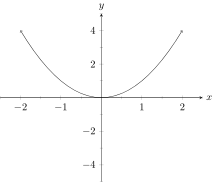
\includegraphics{./Picture01.png}
            }
        \choice{
            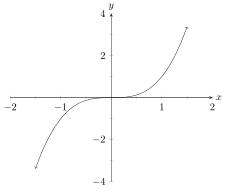
\includegraphics{./Picture02.png}
            }
        \choice{
            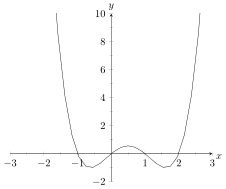
\includegraphics{./Picture03.png}
            }
        \choice{
            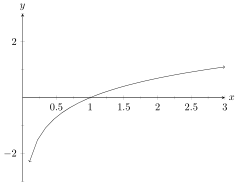
\includegraphics{./Picture04.png}
            }
        \choice[correct]{
            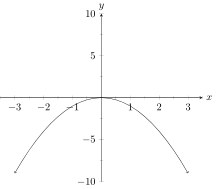
\includegraphics{./Picture05.png}
            }
    \end{multipleChoice}
    \end{problem}





\begin{problem}
    Which of the following graphs would most properly be said to have the parent function $f(x) = e^x$?
    \begin{multipleChoice}
        \choice[correct]{
            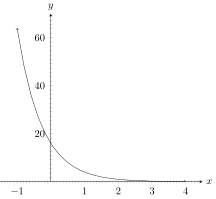
\includegraphics{./Picture06.png}
            }
        \choice{
            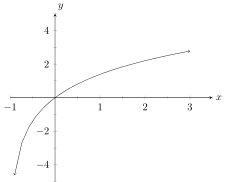
\includegraphics{./Picture07.png}
            }
        \choice{
            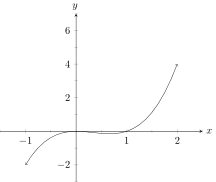
\includegraphics{./Picture08.png}
            }
        \choice{
            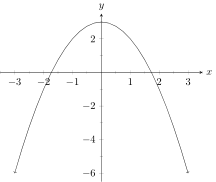
\includegraphics{./Picture09.png}
            }
        \choice{
            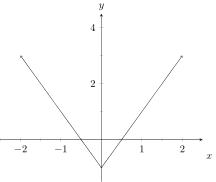
\includegraphics{./Picture10.png}
            }
    \end{multipleChoice}
\end{problem}


\begin{problem}
    Given the following graph:  
    \begin{center}
        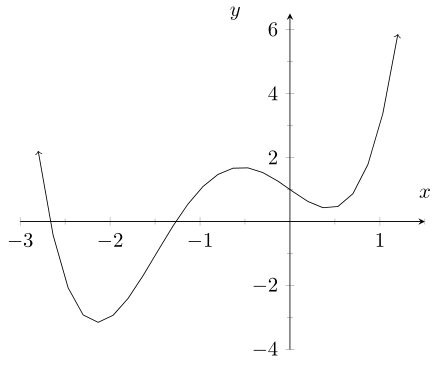
\includegraphics{./Picture11.png}
    \end{center}

    What are the approximate (x,y) coordinates of the local minimum(s), if any exist? (Select all that are local minimums; keep in mind we are asking for an approximation, not precise values)
    \begin{multipleChoice}
        \choice[correct]{$\left(-\frac{9}{4},-\frac{5}{2}\right)$ and $\left( \frac{1}{2}, \frac{1}{4} \right)$}
        \choice{$\left( \frac{1}{2}, \frac{1}{4} \right)$}
        \choice{$\left( -\frac{3}{4}, \frac{19}{10} \right)$}
        \choice{$\left(-\frac{9}{4},-\frac{5}{2}\right)$}
        \choice{There are no local minimums.}
    \end{multipleChoice}
\end{problem}
    
\begin{problem}
    Given the following graph:  
    \begin{center}
        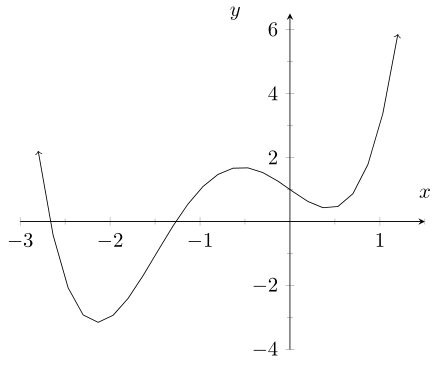
\includegraphics{./Picture12.png}
    \end{center}
    What are the approximate (x,y) coordinates of the absolute maximum(s), if any exist?
    \begin{multipleChoice}
        \choice{$\left(-\frac{9}{4},-\frac{5}{2}\right)$}
        \choice{$\left( \frac{1}{2}, \frac{1}{4} \right)$}
        \choice{$\left( -\frac{3}{4}, \frac{19}{10} \right)$}
        \choice{$\left(\frac{5}{4},6\right)$}
        \choice[correct]{There are no absolute maximums.}
    \end{multipleChoice}
\end{problem}


\begin{problem}
    Given the following graph:  
    \begin{center}
        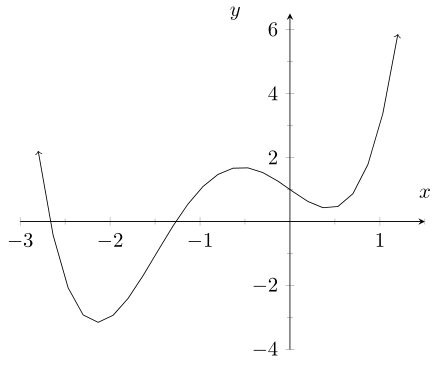
\includegraphics{./Picture13.png}
    \end{center}
    On what interval(s) is the function f(x) decreasing? (Approximate the endpoints if needed.)
    \begin{multipleChoice}
        \choice[correct]{$\left(-\infty, -\frac{9}{4} \right) \cup \left(-\frac{3}{4}, \frac{1}{2} \right)$}
        \choice{$\left(-\frac{9}{4}, -\frac{3}{4} \right)$}
        \choice{$\left(-\frac{3}{4}, \frac{1}{2} \right)$}
        \choice{$\left(-\infty, -\frac{9}{4} \right)$}
        \choice{$\left(\frac{5}{4}, \infty \right)$}
    \end{multipleChoice}
\end{problem}



\begin{problem}
    Consider the following graph:
    
    \begin{center}
        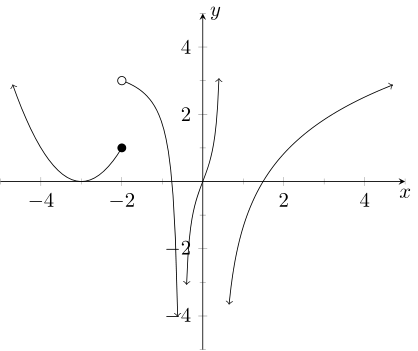
\includegraphics{./Picture14.png}
    \end{center}    
    
    Does the graph have any \textbf{relative} extrema? If so, (approximately) where?
    \begin{multipleChoice}
        \choice[correct]{Yes; a minimum at $(-3,0)$}
        \choice{Yes; a minimum at $(-3,0)$ and a maximum at $(-2,3)$}
        \choice{Yes; a minimum at $(-3,0)$ and a maximum at $(-2,1)$}
        \choice{Yes; a maximum at $(-2,3)$}
        \choice{Yes; a maximum at $(-2,1)$}
    \end{multipleChoice}
\end{problem}

\begin{problem}
    Consider the following graph:
    
    \begin{center}
        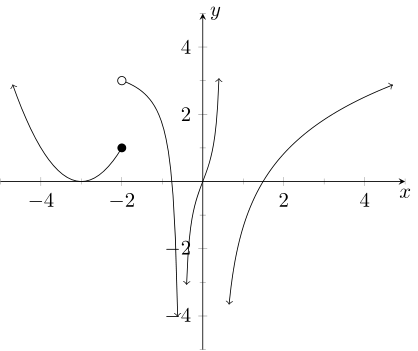
\includegraphics{./Picture15.png}
    \end{center}
    
    Does the graph have any discontinuities? If so, what type?
        \begin{multipleChoice}
        \choice[correct]{Yes, it has both infinite and jump discontinuities.}
        \choice{Yes, it (only) has jump discontinuities.}
        \choice{Yes, it (only) has infinite discontinuities.}
        \choice{Yes, it has jump, infinite, and hole discontinuities.}
        \choice{Yes, it has infinite and hole discontinuities.}
    \end{multipleChoice}
\end{problem}

\begin{problem}
    Consider the following graph:
    
    \begin{center}
        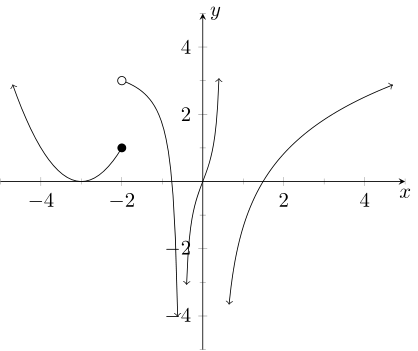
\includegraphics{./Picture16.png}
    \end{center}
    
    Does this graph have any \textbf{absolute} extrema?
    \begin{multipleChoice}
        \choice[correct]{No, because the graph extendws infinitely up and down.}
        \choice{No, because the graph extendws infinitely left and right.}
        \choice{No, because the graph has discontinuities.}
        \choice{Yes, it has an absolute minimum.}
        \choice{Yes, it has an absolute minimum and maximum.}
    \end{multipleChoice}
\end{problem}



\begin{problem}
    Which of the following graphs depicts a continuous relationship?

    \begin{multipleChoice}
        \choice[correct]{
            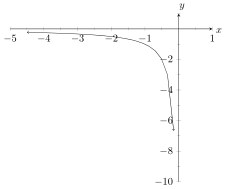
\includegraphics{./Picture17.png}
            }
        \choice{
            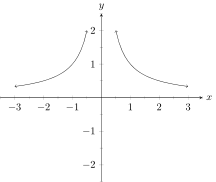
\includegraphics{./Picture18.png}
            }
        \choice{
            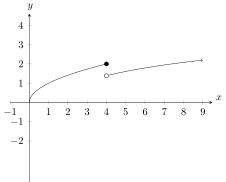
\includegraphics{./Picture19.png}
            }
        \choice{
            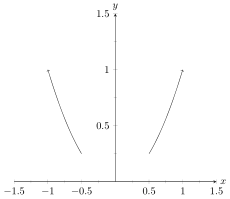
\includegraphics{./Picture20.png}
            }
        \choice{
            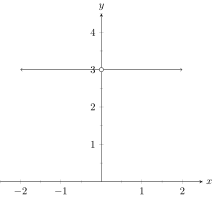
\includegraphics{./Picture21.png}
            }
    \end{multipleChoice}
\end{problem}


\begin{problem}
    Identify the coordinates of the points shown on the graph.
    \begin{center}
        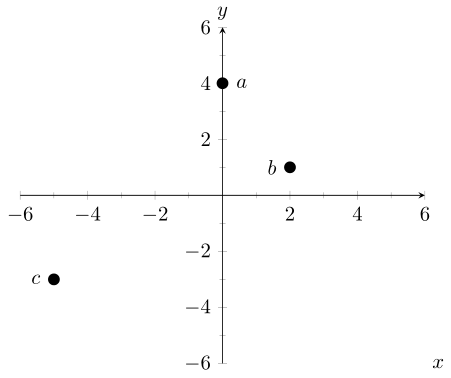
\includegraphics{./Picture22.png}
    \end{center}
    \begin{multipleChoice}
        \choice[correct]{a: (0,4); b: (2,1); c: (-5, -3)}
        \choice{a: (-4,0); b: (-1,2); c: (-3, 5)}
        \choice{a: (0,-4); b: (-2,-1); c: (5, 3)}
        \choice{a: (4,0); b: (1,2); c: (-3,-5)}
        \choice{a: (0,4); b: (-2,1); c: (5, -3)}
    \end{multipleChoice}
\end{problem}



\begin{problem}
    For the following graph which is the correct parent function?
    \begin{center}
        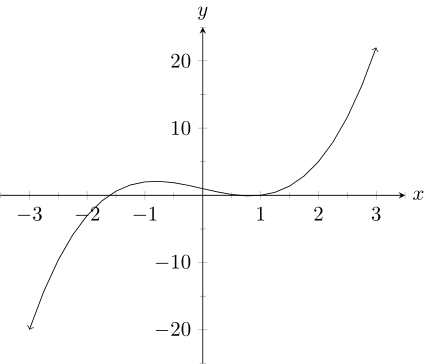
\includegraphics{./Picture23.png}
    \end{center}

    \begin{multipleChoice}
        \choice[correct]{$f(x)=x^3$}
        \choice{$f(x)=x^2$}
        \choice{$f(x) = |x|$}
        \choice{$f(x) = e^x$}
        \choice{$f(x) = \sqrt[3]{x}$}
    \end{multipleChoice}
\end{problem}


\end{document}